% Options for packages loaded elsewhere
\PassOptionsToPackage{unicode}{hyperref}
\PassOptionsToPackage{hyphens}{url}
%
\documentclass[
]{book}
\usepackage{amsmath,amssymb}
\usepackage{lmodern}
\usepackage{iftex}
\ifPDFTeX
  \usepackage[T1]{fontenc}
  \usepackage[utf8]{inputenc}
  \usepackage{textcomp} % provide euro and other symbols
\else % if luatex or xetex
  \usepackage{unicode-math}
  \defaultfontfeatures{Scale=MatchLowercase}
  \defaultfontfeatures[\rmfamily]{Ligatures=TeX,Scale=1}
\fi
% Use upquote if available, for straight quotes in verbatim environments
\IfFileExists{upquote.sty}{\usepackage{upquote}}{}
\IfFileExists{microtype.sty}{% use microtype if available
  \usepackage[]{microtype}
  \UseMicrotypeSet[protrusion]{basicmath} % disable protrusion for tt fonts
}{}
\makeatletter
\@ifundefined{KOMAClassName}{% if non-KOMA class
  \IfFileExists{parskip.sty}{%
    \usepackage{parskip}
  }{% else
    \setlength{\parindent}{0pt}
    \setlength{\parskip}{6pt plus 2pt minus 1pt}}
}{% if KOMA class
  \KOMAoptions{parskip=half}}
\makeatother
\usepackage{xcolor}
\usepackage{longtable,booktabs,array}
\usepackage{calc} % for calculating minipage widths
% Correct order of tables after \paragraph or \subparagraph
\usepackage{etoolbox}
\makeatletter
\patchcmd\longtable{\par}{\if@noskipsec\mbox{}\fi\par}{}{}
\makeatother
% Allow footnotes in longtable head/foot
\IfFileExists{footnotehyper.sty}{\usepackage{footnotehyper}}{\usepackage{footnote}}
\makesavenoteenv{longtable}
\usepackage{graphicx}
\makeatletter
\def\maxwidth{\ifdim\Gin@nat@width>\linewidth\linewidth\else\Gin@nat@width\fi}
\def\maxheight{\ifdim\Gin@nat@height>\textheight\textheight\else\Gin@nat@height\fi}
\makeatother
% Scale images if necessary, so that they will not overflow the page
% margins by default, and it is still possible to overwrite the defaults
% using explicit options in \includegraphics[width, height, ...]{}
\setkeys{Gin}{width=\maxwidth,height=\maxheight,keepaspectratio}
% Set default figure placement to htbp
\makeatletter
\def\fps@figure{htbp}
\makeatother
\setlength{\emergencystretch}{3em} % prevent overfull lines
\providecommand{\tightlist}{%
  \setlength{\itemsep}{0pt}\setlength{\parskip}{0pt}}
\setcounter{secnumdepth}{5}
\usepackage{booktabs}
\ifLuaTeX
  \usepackage{selnolig}  % disable illegal ligatures
\fi
\usepackage[]{natbib}
\bibliographystyle{apalike}
\IfFileExists{bookmark.sty}{\usepackage{bookmark}}{\usepackage{hyperref}}
\IfFileExists{xurl.sty}{\usepackage{xurl}}{} % add URL line breaks if available
\urlstyle{same} % disable monospaced font for URLs
\hypersetup{
  pdftitle={Data Privacy Handbook},
  pdfauthor={Utrecht University \textbar{} Last updated: 2023-02-17},
  hidelinks,
  pdfcreator={LaTeX via pandoc}}

\title{Data Privacy Handbook}
\author{Utrecht University \textbar{} Last updated: 2023-02-17}
\date{17 februari 2023}

\begin{document}
\maketitle

{
\setcounter{tocdepth}{1}
\tableofcontents
}
\hypertarget{part-intro}{%
\part*{Intro}\label{part-intro}}
\addcontentsline{toc}{part}{Intro}

\hypertarget{data-privacy-handbook}{%
\chapter*{Data Privacy Handbook}\label{data-privacy-handbook}}
\addcontentsline{toc}{chapter}{Data Privacy Handbook}

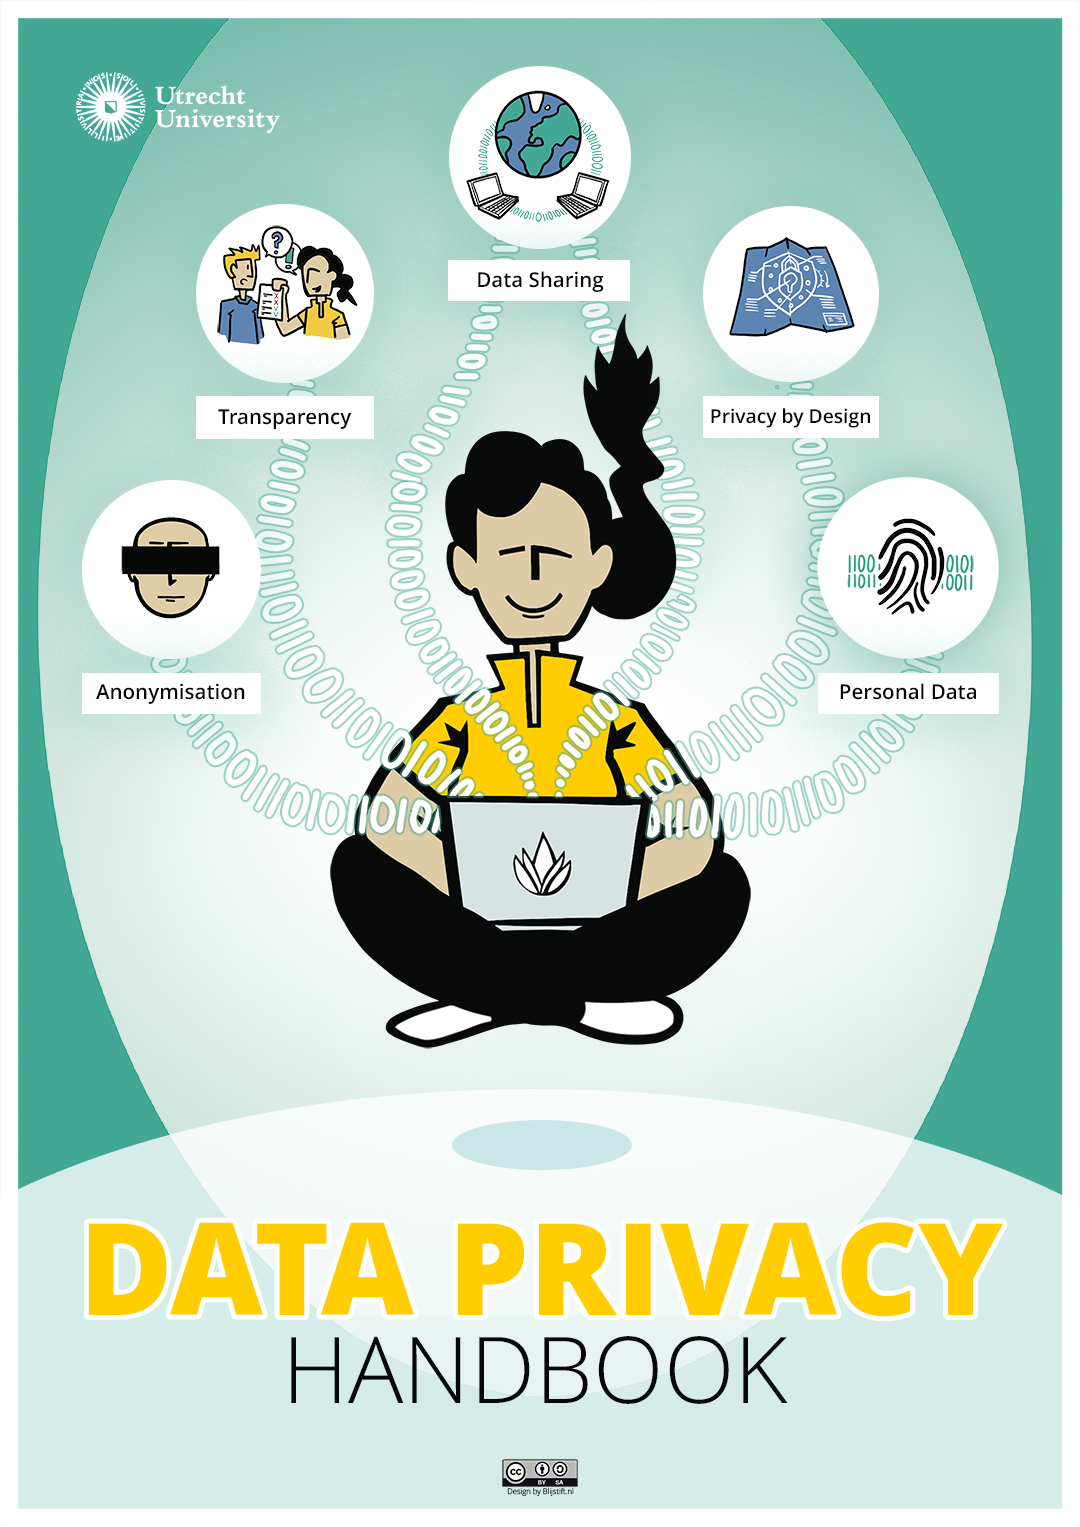
\includegraphics{img/cover-image-dph.png}

\emph{Last updated: 17 February 2023}

The Data Privacy Handbook is a guide on handling personal data in scientific
research, in line with European data protection and privacy regulations. It
consists of:

\begin{itemize}
\tightlist
\item
  A \textbf{knowledge base} which explains how the EU General Data Protection
  Regulation (GDPR, Dutch: Algemene Verordening Gegevensbescherming) applies to
  scientific research, including guidelines and good practices in carrying out
  GDPR-compliant scientific research;
\item
  An overview of privacy-enhancing \textbf{techniques \& tools} and practical guidance
  on their implementation;
\item
  \textbf{Use Cases} in the form of research projects with privacy-related issues,
  for which a reusable solution (e.g., tool, workflow) has been developed.
\end{itemize}

The Data Privacy Handbook synthesises information across various sources and
presents it a \emph{practical} format. This includes workflows, tools, and practical
translations of the GDPR, which could be used by researchers and (data) support
staff within Utrecht University and beyond.

The Data Privacy Handbook is an initiative of
\href{https://www.uu.nl/en/research/research-data-management}{Research Data Management Support},
in collaboration with privacy and data experts at
Utrecht University. It is part of a larger project, the
\href{https://utrechtuniversity.github.io/dataprivacyproject}{Data Privacy Project},
which aims to develop knowledge, tools, and experience
on how researchers can and should deal with personal data. This project is
funded by the Utrecht University Research IT Program and an NWO Digital
Competence Center grant.

This is an Utrecht University (UU) community-driven,
\href{https://github.com/UtrechtUniversity/dataprivacyhandbook}{open source project}.
We welcome feedback and contributions of any type, please read our
\href{https://github.com/UtrechtUniversity/dataprivacyhandbook/blob/main/CONTRIBUTING.md}{contributing guidelines}
for more information.

\hypertarget{how-to-use-this-handbook}{%
\section{How to use this Handbook}\label{how-to-use-this-handbook}}

The Data Privacy Handbook aims to make knowledge and solutions on handling personal
data \emph{Findable, Accessible, Interoperable, and Reusable} (FAIR) and present them in
a practical format.

The Handbook need not be read like a textbook. You are invited to navigate to the
topic you need based on the table of contents, or use the guide below.

\hypertarget{what-are-you-looking-for}{%
\subsection{What are you looking for?}\label{what-are-you-looking-for}}

I want to\ldots:

Learn about the GDPR in the context of scientific research

Introduction to the GDPR

Definitions

Plan a GDPR-compliant research project

Designing your research project

Choosing a legal basis

Assessing the risks in your project,
for example using a privacy scan,
Data Protection Impact Assessment, or
Data classification

Informing participants

Obtaining consent

Collaborating on personal data

Setting up agreements

Work safely with personal data

Storing personal data

Using GDPR-compliant tools and services

De-identifying personal data

Securely computing personal data

Sharing personal data during research

Using other approaches to protect personal data, such as
encryption,
statistical privacy,
synthetic data, or
data donation

Share personal data with others

Sharing data legally

Sharing personal data during research

De-identifying personal data

Securely computing personal data

Using GDPR-compliant tools and services

Sharing personal data for reuse

Sharing personal data case by case

Learn from other projects

Minimising personal data in a survey

Pseudonymising different types of data

Publishing metadata only

Reusing education data for research purposes

Get help or information

Getting help at Utrecht University

Definitions

References

\hypertarget{license-and-citation}{%
\section{License and Citation}\label{license-and-citation}}

The Data Privacy Handbook is licensed under a
\href{https://creativecommons.org/licenses/by/4.0/}{Creative Commons Attribution 4.0 International License}.
You can \href{https://github.com/UtrechtUniversity/dataprivacyhandbook/blob/main/LICENSE.md}{view the license here}.

\hypertarget{disclaimer}{%
\section{Disclaimer}\label{disclaimer}}

The content presented in the Data Privacy Handbook has been carefully curated by
Research Data Management Support, in collaboration with privacy officers and
data experts of Utrecht University.

The Data Privacy Handbook is a `living' book that is continually being written,
updated and reviewed. Its contents can therefore change, or become outdated or
redundant. Hence, the information presented is provided ``as is'', \textbf{without
guarantees of accuracy or completeness}.

As scientific research may differ depending on the discipline, topic, and
context, measures needed or taken to ensure GDPR-compliance will vary across
research projects. The authors can therefore \textbf{not be held responsible, nor
accountable} for any negative consequences arising from interpretation and use
of the content of the Data Privacy Handbook.

The Handbook is not endorsed by the Board of Utrecht University and does not
constitute a mandatory directive. \textbf{For the most up-to-date and official/
authoritative information, please refer to the
\href{https://www.uu.nl/en/research/research-data-management}{university website}
and \href{https://intranet.uu.nl/en/knowledge-base/privacy-at-uu}{intranet},
to which this Handbook is a hands-on, practical supplement}. Moreover, before
implementing the guidance laid out in this Handbook, always seek the advice of
your privacy officer or RDM Support to confirm the suitability of any proposed
solution to your project.

Throughout the Data Privacy Handbook, links to external webpages may be provided
for additional information or assistance. The authors of the Data Privacy
Handbook are \textbf{not responsible for the content of any such linked webpages}, nor
is the content of external webpages necessarily endorsed by Utrecht University.

Utrecht University is committed to sharing knowledge in line with the principles
of open science and therefore welcomes readers from outside of the organization.
However, the contents of the Data Privacy Handbook may not be in line with readers'
institutions' policies or views. For more authoritative information, these
readers should refer to resources from their own institutions.

\hypertarget{contributions}{%
\section{Contributions}\label{contributions}}

The Data Privacy Handbook is a collaborative effort, made possible by a large
number of contributors (also to be viewed in our
\href{https://github.com/UtrechtUniversity/dataprivacyhandbook}{GitHub repository}):

Neha Moopen, Dorien Huijser, Jacques Flores, Mercedes Beltrán, Kasper de Bruijn,
Wies Cipido, Ruud Dielen, David Gecks, Joris de Graaf, Judith de Haan,
Saskia van den Hout, Frans Huigen, Artan Jacquet, Rik Janssen, Sanne Kleerebezem,
Annemiek van der Kuil, Danny de Koning-van Nieuwamerongen,
Pieter Sebastiaan de Lange, Frans de Liagre Böhl, Maisam Mohammadi Dadkan,
Francisco Romero Pastrana, Najoua Ryane, Johanneke Siljee, Maarten Schermer, Raoul Schram,
Ron Scholten, Garrett Speed, Robert Steeman, Jacqueline Tenkink-de Jong,
Liliana Vargas Meleza, and Martine de Vos.

Would you like to contribute to this Handbook yourself? Please read our
\href{https://github.com/UtrechtUniversity/dataprivacyhandbook/blob/main/CONTRIBUTING.md}{Contributing guidelines}.

\hypertarget{faq}{%
\chapter{Privacy FAQs}\label{faq}}

On this page you can find Frequently Asked Questions (FAQs) about handling
personal data in research. Click a question you have to read its answer.

\hypertarget{general}{%
\subsection{General questions}\label{general}}

When should I be dealing with privacy in my project?

You should think about privacy:

as soon as you are processing personal data. Processing means anything you do with personal data, e.g., collecting, analysing, sharing, storing, etc. The definition of personal data is explained in the chapter \protect\hyperlink{personal-data}{What are personal data?}.

during the earliest stages of your project. This principle is called ``\protect\hyperlink{privacy-by-design}{privacy by design}''. It is easier and more effective to address any privacy issues at the design phase of your project rather than having to change your plans later on due to privacy concerns.

When are data truly anonymous?

You can read all about this in the chapters \protect\hyperlink{personal-data}{What are personal data?} and \protect\hyperlink{pseudonymisation-anonymisation}{Pseudonymisation and anonymisation}.

What should I consider when handling personal data?

It is best to conduct a \protect\hyperlink{privacy-scan}{privacy scan} to check if you work with personal data. The below figure summarises what you need to describe, determine and do as part of a privacy scan: 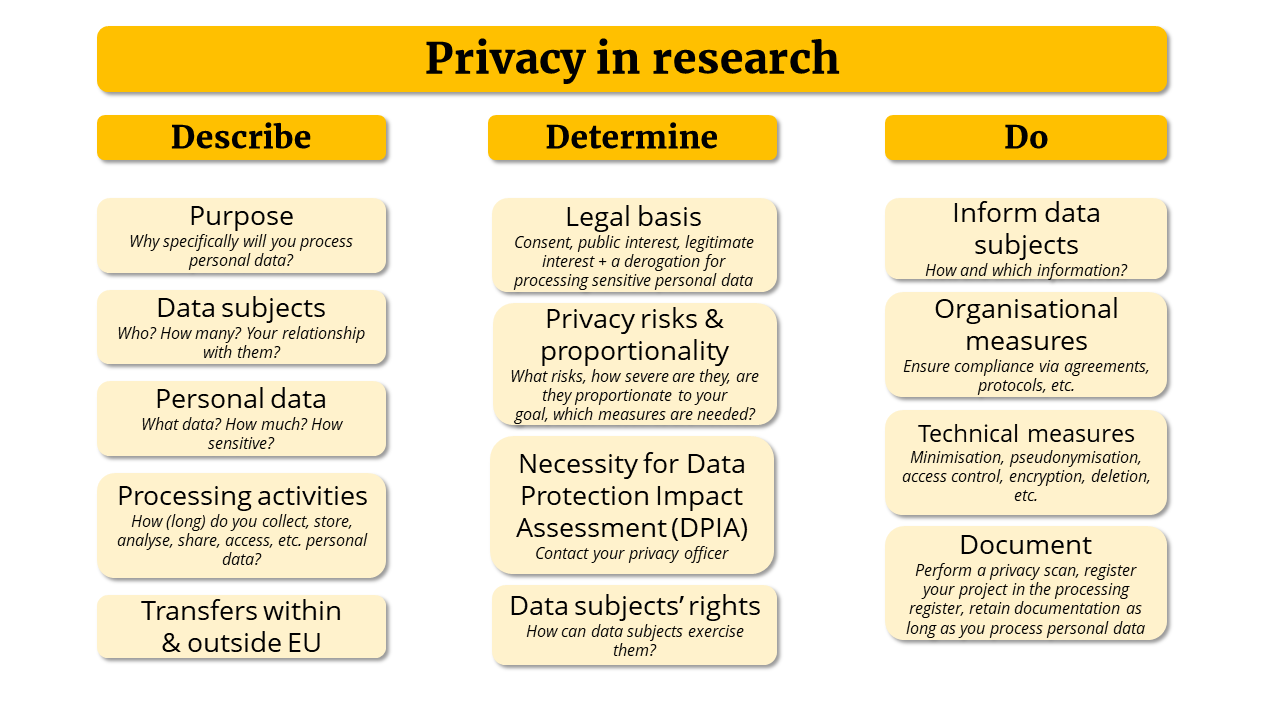
\includegraphics{img/privacyscan_infograph.png}

My data were collected prior to the GDPR, what rules do I need to follow?

The GDPR applies to all personal data, including those collected prior to the GDPR (May 2018). Therefore, there is really no difference between how personal data should be handled before or after the advent of the GDPR.

My data were collected outside of the EU, does the GDPR apply to them?

Yes, as long as personal data are being processed, and the \protect\hyperlink{definitions}{data controller, data processor, or data subject} reside(s) in the European Economic Area, the \protect\hyperlink{gdpr-scope}{GDPR applies}.~

How sensitive are my data?

Personal data can differ in sensitivity, depending on the type of data (e.g., \protect\hyperlink{special-types-personal-data}{sensitive personal data}), of whom the data were collected (e.g., healthy adults, children, patients, elderly, etc.) and on which scale. \protect\hyperlink{data-classification}{Data classification} and a \protect\hyperlink{dpia}{Data Protection Impact Assessment} are useful tools to assess how sensitive the data are.

\hypertarget{procedures}{%
\subsection{Procedures and responsibilities}\label{procedures}}

Who is responsible for correctly handling personal data?

Legally, the \protect\hyperlink{definitions}{controller} of the personal data is responsible, i.e., the people or organisation responsible for the project activities. If you are an employee at Utrecht University (UU), the UU is legally the controller. The UU however delegates this responsibility to the appropriate employee who is actually in charge of determining why and how personal data are handled. In a research context, this is usually the researcher on the project (e.g., PhD candidate, principal investigator).

What does the procedure look like for researchers at Utrecht University?

All researchers at UU have to write a \href{https://www.uu.nl/en/research/research-data-management/guides/data-management-planning}{Data Management Plan}. Besides that, many faculties ~require that a \protect\hyperlink{privacy-scan}{privacy scan} is done and ethical approval is obtained. Preferably, a Data Management Plan and privacy scan (which has to sometimes be extended to a \protect\hyperlink{dpia}{Data Protection Impact Assessment}) are done (and preferably marked as positive by the relevant data steward/privacy officer) before the ethical review takes place. Once accepted by the ethical committee, you can then start your research project.

How long will the planning process ~of my research take?

This differs per faculty, but you should count at least 1 month, if not more, to complete all planning activities. In terms of administrative work, you need to reserve time for:

writing a Data Management Plan and having it reviewed (a few days)

filling out the \protect\hyperlink{privacy-scan}{privacy scan} and consulting with the privacy officer (a few days). If a DPIA needs to be conducted, this will take more time because the Data Protection Officer also needs to be consulted.

creating information for data subjects and potentially a consent form.

going through ethical review: it can take up to 1 month before a first decision is taken by some faculty review boards, or longer for the Medical-Ethical Review Board.

in some projects, setting up an agreement.

In general, designing your research with correctly processing personal data in mind will cost you less effort In the long run: Start as early as possible!

Doesn't the ethical committee also look at privacy?

Partly, although this differs per UU faculty. In most faculties, there is a collaboration between privacy and ethics. For example, at the Faculties of Social and Behavioural Sciences, the Humanities, and Geosciences, privacy is included in the ethical application, but the privacy aspect of it is outsourced to the faculty privacy officer. For you as a researcher, it is wise to first complete a draft \protect\hyperlink{privacy-scan}{privacy scan}, and consult with the faculty privacy officer and only then do the ethical application, so you have already thought about the privacy aspect before the ethical review process starts.

\hypertarget{consent}{%
\subsection{Informed consent}\label{consent}}

When is parental consent needed?

The GDPR dictates that at least one legal guardian provide consent if you process personal data from children under 16 years old. Note that for medical data and in some faculties, there can be additional requirements, such as obtaining written consent from both parents, and also from the child themselves if the child is between 12 and 15 years old.

Can consent be digital?

Yes, as long as you can \protect\hyperlink{forms-consent}{demonstrate} that consent was obtained, it is valid according to the GDPR. Consent can for example consist of participants ticking a checkbox in a survey tool after reading or watching information about the research. The checkbox should be empty at the start of the survey and not already come ``pre-ticked'': consent must be actively given. Note that for \href{https://www.ccmo.nl/onderzoekers/wet-en-regelgeving-voor-medisch-wetenschappelijk-onderzoek/de-wmo-in-een-notendop/toestemming/elektronische-toestemming}{medical data}, consent may have to be provided in writing: always check with your Ethical Review Board.

Where can I find a template consent form?~~~

You can use the \href{https://www.uu.nl/sites/default/files/RDM_Support_Template_Information_letter.pdf}{minimal list of requirements} for an information letter and read through the guidance on \protect\hyperlink{informed-consent-forms}{informed consent} and \protect\hyperlink{privacy-notices}{information to data subjects}. Please note that some \href{https://intranet.uu.nl/en/knowledgebase/ethics-assessment}{Ethical Review Boards} have specific templates that you should use.

How to balance being complete vs.~being intelligible in the information to participants?

The GDPR does not require you to provide all details in the same way to participants. For example, it allows you to layer information, and it requires that you always provide the information in a format that is intelligible for your target audience, which does not necessarily have to be in text. Please refer to the section on \protect\hyperlink{privacy-notices}{Information to data subjects} for more information on this. Please note that some Ethical Review Boards have specific requirements on how information should be provided to participants, which have to do with ethical and legal aspects other than the GDPR.

Where, how and for how long should I store my consent forms?

Consent forms have to be stored securely (access-controlled) and separately from the research data, for as long as the research data contain personal data. This can be in digital or physical (e.g., paper) form. Once the personal data are deleted or fully anonymised, the consent forms should be deleted as well. An empty consent form can be stored for longer, for example to check the phrases about re-use. Read more about this in the \protect\hyperlink{data-storage}{Data storage} chapter.

A participant wants to withdraw their consent. Can I continue to use their data afterwards?

No, once a participant has withdrawn consent, you are obliged to remove any of their data that is under your control and cease any further use of their data from that point onwards. Any processing that occurred \emph{prior} to withdrawal is nevertheless still legal. For example, if the data were published and made publicly available prior to their withdrawal, you are not obliged to take down the entire dataset and seek all individuals that may have downloaded the data subject's data. Another example is if you already analysed the data (but have not yet published the results). In that case, the data have to be deleted, but you do not necessarily need to re-do the analysis. The only important thing is that the data then no longer support the analysis, so for research integrity reasons, you may want to re-do the analysis anyway.Additionally, if you cannot find the participant's data in your dataset because they are deidentified too much, then you are exempt from removing them, unless participants can provide you with information to enable their re-identification.

\hypertarget{legal}{%
\subsection{Legal questions}\label{legal}}

What if I cannot formulate a specific research question in advance?

It is not always possible in research to be very specific about what the personal data will be used for in the future. In some cases, you can therefore use the concept of ``broad consent'', where you continuously inform data subjects and enable them to exercise their rights. This is described \protect\hyperlink{broad-consent}{in more detail here}.

I will move to another institution, can I take my research data that contains personal data with me?

Moving data to another institution constitutes a new way of ``processing'' data and implies that there will be a new (additional) controller of the personal data. This means that you need to take some additional steps, such as ensuring that data subjects are informed about the move, the purpose of the transfer is compatible with the original purpose(s) for data use, both institutions sign an agreement on data protection, use and ownership of the data, etc. What is possible depends largely on the context of your research and the type of data you have: contact your \href{https://intranet.uu.nl/en/knowledgebase/privacyofficers}{faculty privacy officer} for assistance.

When do I have to perform a Data Protection Impact Assessment?

If there is a possibility for a \protect\hyperlink{high-risk-processing}{high risk of damages} to data subjects, a DPIA is mandatory. This can for example be the case when you observe people in public spaces or process sensitive personal data on a large scale. Note that correctly performing a DPIA can take some time. Contact your faculty privacy officer if you suspect that you may need a DPIA.

Do I need an agreement?

An agreement is usually needed when someone outside of your institution accesses (personal) data that you control. Please refer to the \protect\hyperlink{agreements}{Agreements section} to assess whether you need an agreement, and if so, which type.

What is the difference between a Data Transfer Agreement and a Data Processing Agreement?

A data transfer agreement is needed when (personal) data are transferred from one controller to another, and is also recommended to use when data are transferred between departments of a single controller, to delineate the agreed upon responsibilities. For example, in research is it used often when data are shared with other researchers for reuse. A data processing agreement is needed when personal data are transferred from a controller to a processor. For example, it is needed to ensure that an external survey tool protects the university's personal data sufficiently and does not use it for their own purposes, only to provide their survey services. You can read more about \protect\hyperlink{agreements}{these agreements here}.

Am I a processor as employee of my university?

No.~As an employee you are still determining your own why (research question) and how (methods) of personal data processing. This makes you a controller, acting as an ``agent'' of the legal controller (your university). Read more on the difference between processors and controllers \protect\hyperlink{definitions}{on the definitions page}.

\hypertarget{storage}{%
\subsection{Storing personal data}\label{storage}}

Where should I store physical personal data?

Physical personal data should be stored in a locked area that only a select group of people has access to. The exact location will depend on the type of data (e.g., consent forms, filled out questionnaires, biomedical samples, etc.), and where you work. If possible, we recommend digitising and then destroying any paper materials in order to have the data in a secure and backed-up location.

Where to store participants' contact information?

Similarly to informed consent forms, you should store contact information on a different location than the research data and well-protected (strict access control, encryption, etc.). For example, store the research data on Yoda, and the contact information in a controlled OneDrive or ResearchDrive folder. Delete the contact information when you do not longer need them (e.g., after the research project has ended).

\hypertarget{sharing}{%
\subsection{Sharing, publishing and reusing personal data}\label{sharing}}

Can I publish personal data?

This is not only a privacy issue, but also an ethical one. You can in principle ask consent to publish personal data (either publicly or under restricted access), or in some cases rely on public interest to do so. Because the data will remain protected by the GDPR, anyone (re)using the data will have to abide by the GDPR as well (the requirements travel with the personal data). However, even if you have a legal basis to publish personal data, it still may not always be ethical to do so. For that reason, we recommend always obtaining ethical approval, including when you want to publish personal data. You can read more about sharing and publishing personal data for reuse in the \protect\hyperlink{data-sharing-reuse}{Sharing data for reuse chapter}.

How can I share personal data with collaborators?

If the collaborator resides outside of your institute, but within the European Economic Area (EEA) or an \href{https://ec.europa.eu/info/law/law-topic/data-protection/international-dimension-data-protection/adequacy-decisions_en}{``adequate'' country}, it is possible to share personal data with them, provided that data subjects are informed, there is a (joint controllers) \protect\hyperlink{agreements}{agreement} with them, and other safeguards are in place (e.g., pseudonymisation). Please contact your privacy officer if the collaborator is located outside the EEA in a country without an adequate level of data protection.

How can I share data with a third party outside of the EEA?

Personal data can be shared outside of the EEA if one of the following applies:

Participants have given their explicit consent after having been well informed of the risks.

The transfer is necessary for important reasons of public interest.

The data are transferred to a non-EEA country that has been deemed \href{https://ec.europa.eu/info/law/law-topic/data-protection/international-dimension-data-protection/adequacy-decisions_en}{adequate by the European Commission}.

The above apply only to ``occasional'' transfers. For frequent transfers, \protect\hyperlink{scc}{Standard Contractual Clauses} should be drafted, although this requires a greater commitment from the third parties, and may require more in-depth legal assistance to establish.

What should I do if some participants do not consent to sharing their data?

This depends on the identifiability of the data and the legal basis: if it is still possible to identify individuals, then data subjects can withdraw their consent, and you won't be able to share their data for reuse. However, if the data are altered in such a way that you can no longer identify individuals within the dataset, then you can share their data for reuse. Of note, it is not always necessary to ask people their consent for data reuse for scientific purposes - consult your privacy officer. You can read more about this in the \protect\hyperlink{data-sharing-reuse}{Sharing data for reuse} chapter.

Can I reuse medical data for research purposes?

You likely can. The GDPR has a derogation that specifies that secondary use for research is ``not incompatible with the initial purposes'' (\href{https://gdpr-info.eu/art-5-gdpr/}{art. 5(1)(b)}), meaning that it is allowed to reuse data for research, provided that you protect the data sufficiently. As with any research project, we recommend to conduct a \protect\hyperlink{privacy-scan}{privacy scan} to assess the legality of your project, and to obtain ethical approval to assess the ethical aspects of your project.

Can I use personal data that are already published by other researchers?

You generally can, depending on the license or terms of use that the dataset has, and assuming that the researcher who published the data had a legal basis to do so. In general, it is possible to reuse personal data for scientific research, as long as appropriate safeguards are in place (\href{https://gdpr-info.eu/art-89-gdpr/}{art. 89}).

\hypertarget{practical-questions}{%
\subsection{Practical questions}\label{practical-questions}}

I am using hardware to collect personal data. What should I take into account?

There are many security aspects to consider when using hardware (e.g., tablets, cameras, phones, etc.), such as whether and where any personal data is recorded and whether the device is approved by the university, see \href{https://students.uu.nl/en/practical-information/it-facilities/information-security-at-the-uu}{this link} for more information. Make sure that you transfer the data to secure storage as soon as possible and consider measures (such as encryption) that ensure that data are protected if the hardware is lost or stolen. When you use video recording hardware, be mindful of what is recorded, also in the background. For example, be aware when filming around open laptops, documents or vulnerable people.

I want to combine data from multiple sources. How can I do so securely?

There are multiple factors to consider, depending on the type of research, the ownership of the data, involved parties, etc. As a rule of thumb, practice data minimisation, only keep the fields or variables you need. Be mindful of data ownership: if someone else owns the data, keep that dataset separate. For more information and tailored advice, contact \href{https://www.uu.nl/en/research/research-data-management/contact-us}{RDM Support}.

How to generate suitable pseudonyms?

A pseudonym can be a random number, cryptographic hash function, text string, etc. It is important that the pseudonym is not meaningful with respect to the data subjects: a random (unique) number or string is better than a code that contains parts of personal information, because the latter may reveal details about data subjects.

How to pseudonymise qualitative data?

Textual data is often redacted (either manually or using a \href{https://github.com/UtrechtUniversity/privacy-engineering-tools/tree/main/deidentification}{tool} so that identifiable information is removed or replaced with a placeholder text. There are now also tools for masking or blurring video data and distorting audio. Note that sometimes it is not possible to anonymise or pseudonymise qualitative data, because you may lose too much valuable information, or because the data are just too revealing (e.g., face, voice, gestures, posture in video data, language use in audio data). In that case, other measures like access control, safe storage, and encryption may be more suitable.

I am analysing my data in a git repository to ensure reproducibility. How can I make sure I do not accidentally push the data to GitHub?

Before you put your data in your git repository, place a line in the .gitignore file that prevents tracking the data. This way, when pushed to GitHub, the data will not be pushed alongside the other files in the repository - only the folder name will be visible. Please note that if the data were tracked by git before, adding a line to your .gitignore will not prevent the data from being tracked. In this case, it is best to create a new git repository where you add a .gitignore file from the start, and delete all old versions from GitHub if there were any. If you delete the data, add the line to the .gitignore file, and then re-add the dataset, the tracking history from before the .gitignore will still exist and be pushed to GitHub. Sidenote: it is possible to override the .gitignore file by force. This will likely not happen accidentally, but it is important to realise that the .gitignore file is not iron clad. You can read \href{https://the-turing-way.netlify.app/project-design/sdpw/pd-sdp-sensitive-files.html}{more on the gitignore here}.

How to securely send participant data to participants?

In the same protected way as when you would send personal data to fellow researchers. Researchers at Utrecht University can for example use \href{https://filesender.surf.nl/}{SURF filesender} with encryption or share a OneDrive or Research Drive file. Be sure not to share any data from other participants or other researchers!

How to work responsibly with social media data?

See \href{https://doi.org/10.33540/1874/406645}{these guidelines} (in Dutch) about working with social media data. Every social media platform has different terms and conditions. Read these to see what you are, and are not, allowed to do with the data published on the platform you wish to research.

Where can I find relevant or approved tools?

Researchers at Utrecht University can find tools via \url{https://tools.uu.nl} and the \href{https://intranet.uu.nl/en/knowledgebase/software-at-work-teaching-rooms-and-home}{intranet}. We also curated an overview of several tools to handle personal data in \href{https://github.com/UtrechtUniversity/privacy-engineering-tools/}{this GitHub repository}.

Where can I find privacy-related templates and examples for research?

Please refer to the \protect\hyperlink{legal-documents}{Documents and agreements chapter} or the \href{https://www.uu.nl/rdm}{RDM website}. For others, please contact your \href{https://intranet.uu.nl/en/knowledgebase/privacyofficers}{privacy officer} and/or your \href{https://intranet.uu.nl/en/knowledgebase/ethics-assessment}{Ethical Review Board}.

\hypertarget{students}{%
\subsection{Students and student data}\label{students}}

Can I reuse educational data (e.g., grades, course evaluations) for my research?

It is possible, but its compliance would have to be documented in a \protect\hyperlink{privacy-scan}{privacy scan} to explain why this further processing for scientific purposes is compliant with the GDPR. Please refer to the \protect\hyperlink{reuse-education-data}{use case about this topic} for an example.

Can I share my research data containing personal data with my students?

Preferably not. Especially in a classroom setting, students should work on anonymised data as much as possible. For thesis students, only share personal data with them as strictly necessary and make sure that the students know how to safely handle the personal data. Additionally, data subjects should be informed that these students will handle their data.

Can I (re)use personal data collected by my students?

You should check what information was given to data subjects to see whether it is possible to reuse the data. In general, if data are deidentified and are going to be used for research, it is possible to make this data reuse legitimate - a \protect\hyperlink{privacy-scan}{privacy scan} may be able to demonstrate this.

When students collect personal data, who is responsible for correct handling of those data?

The supervisor is the main person responsible, but students are also co-responsible, especially if they are taking decisions on the data themselves. Students need to comply with their respective obligations and responsibilities to ensure data is kept safe and protected.

Can a student take research data containing personal data with them to publish about them later?

It depends on why this is considered necessary, if data subjects have been informed, if data minimisation and deidentification are applied, etc. If students take data with them, they will probably end up being stored on a free cloud solution such as Google Drive or Dropbox. Make sure your data subjects are informed about this beforehand and realise that obtaining consent will be more difficult. A \protect\hyperlink{privacy-scan}{privacy scan} should document why this is compliant with the GDPR.

I am a student, where can I store my data?

If you are student who will be collecting personal data for research, it is the responsibility of your supervisor or course coordinator to supply you with access to an approved storage solution. Please do not use a personal device or commercial cloud solutions like Dropbox or Google Drive to store research data containing personal data. Any ``free'' commercial solution will scrape and analyse what you store and thus your data are not safe there.

\hypertarget{finding-support}{%
\subsection{Finding support}\label{finding-support}}

Where can I learn more?

For Utrecht University researchers, the most relevant information and support can be found here:

\href{https://www.uu.nl/en/research/research-data-management/training-workshops/handling-personal-data-in-research}{Workshop handling personal data}

E-learning Privacy basics for researchers (coming soon)

\href{https://www.uu.nl/rdm}{RDM Support website}

Faculty-specific web pages:

Geosciences: \href{https://geo-data-support.sites.uu.nl/}{RDM and privacy}, \href{https://sciencegeo-erb.sites.uu.nl/}{ethics}

Science: \href{https://science-data-support.sites.uu.nl/}{RDM and privacy}, \href{https://sciencegeo-erb.sites.uu.nl/}{ethics}

Social and Behavioural Sciences: \href{https://techsupport.fss.uu.nl/}{tech support}, \href{https://ferb.sites.uu.nl/}{ethics}

Humanities: \href{https://cdh.uu.nl/research/data-management-privacy/}{RDM and privacy}, \href{https://fetc-gw.wp.hum.uu.nl/}{ethics}

Law, Economics and Governance: \href{https://intranet.uu.nl/en/knowledgebase/facultys-ethical-review-committee}{ethics}

Veterinary medicine: \href{https://www.uu.nl/en/node/589/onderzoeksbureauresearch-support-office}{Research Support Office}

Medicine: \href{https://www.metc-utrecht.nl/en/}{ethics}

Intranet pages on \href{https://intranet.uu.nl/en/knowledge-base/privacy-at-uu}{privacy} and \href{https://intranet.uu.nl/en/knowledgebase/research}{research}

Who is the Data Protection Officer (DPO)?

The Data Protection Officer (Dutch: Functionaris Gegevensbescherming, FG) oversees an organisation's compliance to the General Data Protection Regulation (GDPR). In research, the DPO is sometimes involved in a \protect\hyperlink{dpia}{Data Protection Impact Assessment} and in some cases in possible data breaches. If you work at Utrecht University, you can read more about the \href{https://intranet.uu.nl/en/knowledgebase/data-protection-officer}{DPO's role here}.

I have a potential data breach, what should I do?

If you work or study at Utrecht University, please report this as soon as possible to the \href{https://intranet.uu.nl/en/security/information-security-computer-misuse-or-report-incident-cert}{Computer Emergency Response Team} (CERT).

\hypertarget{part-knowledge-base}{%
\part*{Knowledge Base}\label{part-knowledge-base}}
\addcontentsline{toc}{part}{Knowledge Base}

\hypertarget{gdpr}{%
\chapter*{The GDPR}\label{gdpr}}
\addcontentsline{toc}{chapter}{The GDPR}

\textbf{This chapter will present the most important definitions, principles and rights
of data subjects outlined in the GDPR and how it applies to your research. Most
of the practical advice that we provide in this Handbook will be rooted in and
builds on the concepts presented here.}

\hypertarget{chapter-summary}{%
\subsection{Chapter summary}\label{chapter-summary}}

The GDPR is a EU-wide regulation that controls the processing of personal data.
If you process personal data, you should:

\begin{itemize}
\tightlist
\item
  Make sure you have a \protect\hyperlink{legal-basis}{legal basis} to process the
  data. In research, this is often informed consent.
\item
  Be transparent and fair towards data subjects.
\item
  Be specific in which personal data you process and for what purposes. Limit
  the amount of data you process to what is necessary, and only store the data
  for that necessary amount of time.
\item
  Protect the confidentiality of the data by incorporating
  \protect\hyperlink{privacy-by-design}{privacy by design} into your project from the start.
\item
  Make sure your data subjects can exercise their
  \protect\hyperlink{data-subject-rights}{data subjects' rights}, and they know how to do so.
\end{itemize}

\hypertarget{what-is-the-gdpr}{%
\section{What is the GDPR?}\label{what-is-the-gdpr}}

The General Data Protection Regulation (GDPR, Dutch: \emph{Algemene Verordening
Gegevensbescherming} {[}AVG{]}) is an EU-wide regulation meant to protect the privacy
of individuals within a rapidly growing technological society. The GDPR facilitates
the free movement of personal data within the European Economic Area (EEA). Its
data processing principles are meant to ensure a fair balance between competing
interests -- for example, the right to conduct research vs.~the right to protect
personal data (Articles 13 and 8, from the Charter of Fundamental right of the EU).

\hypertarget{the-gdpr-in-a-nutshell}{%
\subsubsection{The GDPR in a nutshell}\label{the-gdpr-in-a-nutshell}}

All articles and recitals of the GDPR can be found online via \url{https://gdpr-info.eu/}.
The video below highlights some important aspects of the GDPR:

Click to read the English video transcript

The General Data Protection Regulation (GDPR) regulates what we can
and cannot do with personal data such as a person's name, sexual orientation,
home address and health. This also applies to personal data used in research
and education. The regulation consists of 88 pages. Fortunately, the basics
are easy to remember in 3 steps:

First, there must be a clear legal basis for processing personal data. This can
include consent, a legal obligation, or public interest.

Second, appropriate technical and organisational measures must be taken
while processing personal data to ensure maximum privacy.

Lastly, the persons whose data you have collected must always have the
option of inspecting, changing, or removing their personal data.

That is the GDPR in a nutshell.

\hypertarget{gdpr-scope}{%
\subsubsection{When does the GDPR apply?}\label{gdpr-scope}}

The GDPR has been applicable from May 2018 onward and applies when:

\begin{itemize}
\tightlist
\item
  you are processing \protect\hyperlink{personal-data}{personal data}
  (material scope, \href{https://gdpr-info.eu/art-2-gdpr/}{art 2}).
\item
  the controller or processor of the data \emph{resides} in the EEA (territorial
  scope, \href{https://gdpr-info.eu/art-3-gdpr/}{art. 3}).
  This is independent of whether the actual processing takes place in the EEA.
  In some cases, the GDPR also applies when the controller or processor is not
  established in the EEA, but is processing data from EU citizens.
\end{itemize}

If you are collecting or using data that originated from individuals (or is
related to individuals), it is very likely that the GDPR applies to your project.
You can read more in the chapter \protect\hyperlink{personal-data}{What are personal data?}.

\hypertarget{implementation}{%
\subsubsection{Implementation}\label{implementation}}

While the GDPR is a regulation for the entire EEA, each EEA country can additionally
implement further restrictions and guidelines in national implementation laws. The
Dutch implementation law is called
``\href{https://wetten.overheid.nl/BWBR0040940/2021-07-01\%22}{Uitvoeringswet AVG (UAVG)}''.
The UAVG determines, for example, that it is forbidden to process Citizen
Service Numbers (BSN), unless it is for purposes determined by a law or a
General Administrative Order (AMvB).

\hypertarget{definitions}{%
\section{Definitions in the GDPR}\label{definitions}}

Below, you will find a selection of important terms in the GDPR that you should
become familiar with when working with personal data (also included in the
\protect\hyperlink{glossary}{Glossary}). Click a term to see the definition.

Data subject

A living individual who can be identified directly or indirectly through
personal data. In a research setting, this would be the individual whose
personal data is being processed (see below for the definition of processing).

Personal data

Any information related to an identified or identifiable (living) natural
person. This can include identifiers (name, identification number, location
data, online identifier or a combination of identifiers) or factors specific
to the physical, physiological, genetic, mental, economic, cultural or social
identity of the person. Moreover, IP addresses, opinions, tweets, answers to
questionnaires, etc. may also be personal data, either by itself or through a
combination of one another.

Of note: as soon as you collect data related to a person that is identifiable,
you are processing personal data. Additionally, pseudonymised data is still
considered personal data. Read more in
\protect\hyperlink{personal-data}{What are personal data?}.

Special categories of personal data

Any information pertaining to the data subject which reveals any of the below categories:

racial or ethnic origin

political opinions

religious or philosophical beliefs

trade union membership

genetic and biometric data when meant to uniquely identify someone

physical or mental health conditions

an individual's sex life or sexual orientation

The processing of these categories of data is prohibited, unless one of
the exceptions of \href{https://gdpr-info.eu/art-9-gdpr/}{article 9}
applies. For example, an exception applies when:

the data subject has provided explicit consent to process these data for
a specific purpose,

the data subject has made the data publicly available themselves,

processing is necessary for scientific research purposes.

Contact your \protect\hyperlink{support}{privacy officer} if you wish to process special categories of personal data.

Processing

Any operation performed on personal data. This includes collection, storage,
organisation, alteration, analysis, transcription, sharing, publishing, deletion, etc.

Controller

The natural or legal entity that, alone or with others, determines or has an
influence on why and how personal data are processed. On an
organisational level, Utrecht University (UU) is the controller of personal
data collected by UU researchers and will be held responsible in case of GDPR
infringement. On a practical level, however, researchers (e.g., Principal
Investigators) often determine why and how data are processed, and are thus
fulfilling the role of controller themselves.

Note that it is possible to be a controller without having access to personal
data, for example if you assign an external company to execute research for
which you determined which data they should collect, among which data subjects,
how, and for what purpose.

Processor

A natural or legal entity that processes personal data on behalf of the
controller. For example, when using a cloud transcription service, you often
need to send personal data (e.g., an audio recording) to the transcription
service for the purpose of your research, which is then fulfilling the role
of processor. Other examples of processors are mailhouses used to send emails
to data subjects, or Trusted Third Parties who hold the keyfile to link
pseudonyms to personal data. When using such a third party, you must have a
\protect\hyperlink{data-processing-agreement}{data processing agreement} in place.

Legal basis

Any processing of personal data should have a valid legal basis. Without it,
you are now allowed to process personal data at all. The GDPR provides 6 legal
bases which are explained further \protect\hyperlink{legal-basis}{in this chapter}.

Anonymous data

Any data where an individual is irreversibly de-identified, both directly
(e.g., through names and email addresses) and indirectly. The latter means
that you cannot identify someone:

by combining variables or datasets (e.g., a combination of date of birth,
gender and birthplace, or the combination of a dataset with its name-number key)

via inference, i.e., when you can deduce who the data are about (e.g.,
when profession is Dutch prime minister, it is clear who the data is about)

by singling out a single subject, such as through unique data points
e.g., someone who is 210 cm tall is relatively easy to identify)

Anonymous data are no longer personal data and thus not subject to GDPR
compliance. In practice, anonymous data may be difficult to attain and care
must be given that the data legitimately cannot be traced to an individual in
any way. The document
\href{https://ec.europa.eu/justice/article-29/documentation/opinion-recommendation/files/2014/wp216_en.pdf}{Opinion 05/2014 on Anonymisation Techniques}
explains the criteria that must be met for data to be considered anonymous.

Pseudonymous data

Personal data that cannot lead to identification without additional
information, such as a key file linking pseudonyms to names. This additional
information should be kept separately and securely and makes for
de-identification that is reversible. Data are sometimes pseudonymised by
replacing direct identifiers (e.g., names) with a participant code (e.g.,
number). However, this may not always suffice, as sometimes it is still
possible to identify participants indirectly (e.g., through linkage, inference
or singling out). Importantly, pseudonymous data are still personal data and
therefore must be handled in accordance with the GDPR.

\hypertarget{gdpr-principles}{%
\section{Principles in the GDPR}\label{gdpr-principles}}

\textbf{The GDPR has a number of principles at its core which dictate the (method of)
data processing. Every type of processing has to comply with these principles.
Understanding these principles is the first step to determining what type of
personal data can be collected and how they can processed.}

The GDPR principles are explained further below the image. The
\protect\hyperlink{privacy-by-design}{Design chapter} describes how to implement these principles
in your research. You can also always contact your \protect\hyperlink{support}{privacy officer}.

\hypertarget{lawful-fair-and-transparent}{%
\subsubsection{1. Lawful, fair and transparent}\label{lawful-fair-and-transparent}}

When working with personal data, your processing should be:

Lawful

Make sure all your processing activities (e.g., data collection, storage,
analysis, sharing) have a \protect\hyperlink{legal-basis}{legal basis}. Ideally,
you should have determined your processing purposes (e.g., research questions)
in advance.

Fair

Consider the broad effects of your processing on the rights and dignity of the data subject.

Give data subjects the possibility to exercise \protect\hyperlink{data-subject-rights}{their rights}.

Avoid deception in the communication with data subjects: processing of personal data should be in line with what they can expect.

The processing of personal data should not have a disproportionate negative, unlawful, discriminating or misleading effect on data subjects.

Transparent

Be transparent in the \protect\hyperlink{privacy-notices}{communication to your data subjects}
about who is processing the personal data (controllers, processors), which
personal data are processed, as well as why and for how long, and how data
subjects can exercise their rights. The information provided should be
unambiguous, concise, easily accessible and relevant and shared with data
subjects before the start of your research.

\hypertarget{purpose-limitation}{%
\subsubsection{2. Purpose limitation}\label{purpose-limitation}}

You can only process (i.e., collect, analyse, store, share, etc.) personal data
for a specific purpose and only for as long as necessary to complete that purpose.
For example, if you communicated to data subjects that you would use their
personal data only to answer your specific research question, you cannot further
share the personal data for new research questions, as these would be additional
processing purposes. This means that you need to \textbf{plan what you will do with
the (collected) personal data in advance and stick to that plan in order to be
GDPR-compliant}.

\hypertarget{data-minimisation}{%
\subsubsection{3. Data minimisation}\label{data-minimisation}}

You can only process the personal data you need to for your predefined purpose(s),
and not more just because they may ``come in handy later''. This principle makes
sure that, for example, in the event of a data breach, the amount of data exposed
is kept to a minimum.

\hypertarget{accuracy}{%
\subsubsection{4. Accuracy}\label{accuracy}}

The accuracy of personal data is integral to data protection. Inaccurate data
can be a risk for data subjects, for example when they lead to a wrong treatment
in a medical trial. You therefore need to take every reasonable step to remove
or rectify data that is inaccurate or incomplete. Moreover, data subjects have
the \protect\hyperlink{data-subject-rights}{right} to request that inaccurate or
incomplete data be removed or rectified within 30 days.

\hypertarget{storage-limitation}{%
\subsubsection{5. Storage limitation}\label{storage-limitation}}

You can only \protect\hyperlink{data-storage}{store personal data} for as long as is
necessary to achieve your (research) purpose. Afterwards, they need to be
removed. If the personal data are part of your research data (and not, for
example, to simply contact data subjects), you are allowed to store (archive)
them for a longer period of time, provided necessary safeguards are in place.
This is an exemption that applies to data storage for scientific archiving
purposes. You need to inform the data subjects on this storage duration beforehand.

If identification of the data subject is no longer needed for your
(research) purposes, you do not need to keep storing the personal data just
to comply with the GDPR, even if it means your data subjects cannot exercise
their rights (\href{https://gdpr-info.eu/art-11-gdpr/}{art. 11}).

\hypertarget{integrity-and-confidentiality}{%
\subsubsection{6. Integrity and confidentiality}\label{integrity-and-confidentiality}}

You have to process personal data securely and protect against unauthorised
processing or access, loss or damage. To this end, you should put in place
apropriate \protect\hyperlink{privacy-by-design}{organisational and technical measures}.

\hypertarget{accountability}{%
\subsubsection{7. Accountability}\label{accountability}}

The controller is ultimately responsible for demonstrating GDPR-compliance. As a
researcher working with personal data, you are representing your institution
(e.g., Utrecht University) and you should therefore be able to demonstrate that
you process personal data in a compliant manner. Additionally, you should also
have some knowledge of data protection so that you can implement the right
measures into your research project.

\hypertarget{legal-basis}{%
\section{Legal bases for working with personal data}\label{legal-basis}}

You can only process personal data if you have a \textbf{legal basis} to do so, which
should be registered, among other information, in the
\protect\hyperlink{processing-register}{processing register} and
\protect\hyperlink{privacy-notices}{communicated to data subjects}. There are 6 possible
legal bases which are outlined below. In research, the legal bases `informed
consent', `public interest' and to some extent `legitimate interests of the
controller' are most often used.

\textbf{For different purposes in your research project, a different
legal basis may apply}. For example, you may contact data subjects before they
start participating based on a legitimate interest and use informed consent for
collecting, storing, analysing and publishing the data.

\hypertarget{legal-bases-suitable-for-research}{%
\subsection{Legal bases suitable for research}\label{legal-bases-suitable-for-research}}

Informed consent

Informed consent is the most frequently used legal basis in research and
is often not only a legal (GDPR-consent), but also an ethical obligation
(e.g., METC informed consent). When using informed consent, you should
be able to demonstrate that the data subject was informed and has given
consent, and for which purpose(s) they gave their consent. In all cases,
consent has to be freely given, specific, informed and unambiguous. Please
refer to the \protect\hyperlink{informed-consent-forms}{Informed consent section} for
guidance on applying informed consent in your research.

Public interest

Public interest is sometimes used in research when the research is shown
to clearly benefit the public good or fulfills a public task. In
essence, public interest can be used for research that is conducted by
employees of public institutions, when their research interest has been
recognised by an official authority. For example, conducting research at
Dutch universities has been officially recognised in the
\href{https://wetten.overheid.nl/BWBR0005682/2022-01-01}{Higher Education and Scientific Research Act}
to be a public task. Public interest is often used when consent is not
a good option. For example, it may be impossible or impractical to
obtain consent when performing public observations or social media
research. Or when participants actually do not have a free choice, such
as in clinical trials when participants would experience significant
disadvantages when not participating.

If you want to use public interest as a legal basis, you
need to assess the necessity and proportionality of your processing.
Additionally, you need to demonstrate that the interests of data
subjects do not override your research interests. To do so, please contact
your \protect\hyperlink{support}{privacy officer} to assess whether you can use this
legal basis in your research.

Legitimate interest of the controller

Legitimate interest is often used by companies to process personal data
necessary for the functioning of their own company, e.g., processing
user data for fraud prevention, or keeping a registration system to
provide better services. In research, legitimate interest is often used
for processing activities that have no direct research purpose. For
example, this can be the case when you need to collect contact
information to approach data subjects to participate, and you can only
obtain their consent for participating in your research after contacting
them. Since contacting data subjects is a prerequisite to perform your
research, it can be in the university's legitimate (research) interest
to process their contact information.

To evaluate whether you can use legitimate interest as a legal basis, you
always need to weigh the interests of the controller (e.g., Utrecht
University) and the data subjects in a
\protect\hyperlink{legitimate-interest-assessment}{Legitimate interest assessment}.
Please contact your \protect\hyperlink{support}{privacy officer} to assess whether you
can use this legal basis in your research.

\hypertarget{legal-bases-not-suitable-for-reseach}{%
\subsection{Legal bases not suitable for reseach}\label{legal-bases-not-suitable-for-reseach}}

Processing is necessary because of a legal obligation of the controller

This basis is not suitable for research. As an example, Utrecht
University has to share tax data with the Dutch tax administration in
order to comply with tax legislation.

Processing is necessary for the performance of a contract

This basis is not suitable for research. As an example, Utrecht
University has contracts with its employees, which require it to manage
the employees' financial data.

Processing is necessary to protect a person's vital interests

This basis is generally not suitable for research. If processing
someone's personal data is crucial to their health or even life, that
processing is allowed under the GDPR.

\hypertarget{further-processing}{%
\subsection{Further processing for research purposes}\label{further-processing}}

It may happen that you want to process personal data for other purposes than
previously specified (e.g., because you formulated an additional research
question), or you want to reuse previously collected personal data in your
research. In these cases, it may be possible to make use of
\href{https://gdpr-info.eu/art-5-gdpr/}{article 5(1)(b)},
which states that ``further processing for {[}\ldots{]} scientific purposes shall {[}\ldots{]}
not be considered to be incompatible with the initial purposes''. Basically, this
means that you can reuse personal data, that were previously collected for other
purposes, for scientific research purposes. This is only allowed if you put in
place sufficient safeguards to protect the personal data, inform data subjects,
and allow them to exercise their rights
(\href{https://gdpr-info.eu/art-89-gdpr/}{art. 89}).
``Further processing'' is not strictly a legal basis. Instead, it functions as a
way to legitimise \emph{further} processing of personal data (which was previously
collected for a different purpose, using one of the six legal bases) for research
purposes.

Public interest, legitimate interest, and relying on further processing are ways
to meet your \emph{legal} requirements for processing personal data, but not
necessarily your \emph{ethical} requirements: you may still need consent if demanded
so from an ethical perspective. Before you rely on any of these, you should
first assess whether they are indeed suitable with your faculty \protect\hyperlink{support}{privacy officer},
and determine whether your research interests outweigh the privacy rights of
the data subjects.

\hypertarget{data-subject-rights}{%
\section{Data Subjects' Rights}\label{data-subject-rights}}

The GDPR provides data subjects with several rights that gives them a relatively
high degree of control over their own personal data. Below, we list these rights
and how you can apply them in your research:

Right to be informed

Data subjects need to be clearly informed about what you are doing with their
personal data (a.o. \href{https://gdpr-info.eu/art-12-gdpr/}{art. 12}).
This usually happens via an \protect\hyperlink{privacy-notices}{information letter}. This right
does not apply if your research will be seriously harmed by meeting it and if
you haven't obtained the personal data directly from the data subjects themselves.

Right of access

Data subjects have the right to access a copy of the personal data you have
on them and to know what you are doing with that personal data and why
(\href{https://gdpr-info.eu/art-15-gdpr/}{art. 15}).

Right to rectification

Data subjects have the right to correct and complement the personal data
that you have of them
(\href{https://gdpr-info.eu/art-16-gdpr/}{art. 16}).

Right to erasure/Right to be forgotten

Data subjects have the right to have their personal data removed (i.e.,
equivalent to the right to withdraw consent,
\href{https://gdpr-info.eu/art-17-gdpr/}{art. 17}).
This right does \textbf{not} need to be granted if:

the personal data are published and need to be archived for validation
purposes.

it would seriously obstruct the research purpose(s).

it would hinder complying with a legal obligation or carrying out a task
in the public interest.

If the personal data have already been made public or shared, you need to
take reasonable measures to inform other users of the data of the erasure
request. A \protect\hyperlink{support}{privacy officer} can help you with this.

Right to restriction of processing

Data subjects have the right to have you process less of their personal data
(\href{https://gdpr-info.eu/art-18-gdpr/}{art. 18}),
for example if their personal data are inaccurate or your processing of it
is unlawful or no longer needed.

Right to data portability

Data subjects have the right to have their personal data transferred to
another party in a ``structured, commonly used and machine-readable format''
(\href{https://gdpr-info.eu/art-20-gdpr/}{art. 20}).

Right to object

Data subjects have the right to object to what you are doing with their
personal data. This right applies when the processing is based on legitimate
or public interest (\href{https://gdpr-info.eu/art-21-gdpr/}{art. 21}).
In case of objection, you have to stop your processing activities and thus
delete any data you have from the particular data subject, unless you can
demonstrate concrete grounds for overriding the data subject's rights
(e.g., excluding the data subject would substantially bias your results).

\hypertarget{how-can-data-subjects-exercise-their-rights}{%
\subsubsection{How can data subjects exercise their rights?}\label{how-can-data-subjects-exercise-their-rights}}

Data subjects need to be \textbf{informed} about their rights and who to contact in
order to exercise them, including when you use a legal basis other than informed
consent. In research, this is usually done via a
\protect\hyperlink{privacy-notices}{privacy notice or information letter}, which states
a contact person responsible for handling questions and requests.

Incoming requests need to be \textbf{coordinated with a privacy officer}, so that
they can be picked up in accordance with the GDPR. Additionally, at Utrecht
University, data subjects can always contact
\href{mailto:fg@uu.nl}{\nolinkurl{fg@uu.nl}} (the Data Protection Officer) for
requests or complaints.

\hypertarget{what-to-do-when-receiving-a-request-concerning-data-subjects-rights}{%
\subsubsection{What to do when receiving a request concerning data subjects' rights?}\label{what-to-do-when-receiving-a-request-concerning-data-subjects-rights}}

You have to provide a substantive response to the data subject \textbf{within 30 days},
in the same way as you received the request. Depending on the complexity and
number of requests, the response period may be extended by 2 months. In that
case, you must inform the data subject about this extension (including the
motivation) within one month. If needed, you can (and sometimes should) ask for
additional information to confirm the data subject's identity.

For granting requests about data subjects' rights, there should be a procedure
in place, in which you should at least consider:

\begin{itemize}
\tightlist
\item
  how you are going to retrieve the data (e.g., using a name-number key)
\item
  who is responsible for granting the request and informing the data subject
  about it (e.g., a data manager)
\item
  how the request is going to be granted, for example how they will be sent
  securely (access, portability), removed (forgotten, object, restriction) or
  corrected (rectification)
\end{itemize}

For larger projects, it may be wise to put a Standard Operating Procedure (SOP)
in place.

\hypertarget{what-if-the-data-have-already-been-anonymised}{%
\subsubsection{What if the data have already been anonymised?}\label{what-if-the-data-have-already-been-anonymised}}

The principles of data minimisation and storage limitation are considered more
important than keeping personal data just for the sake of identification
(\href{https://gdpr-info.eu/art-11-gdpr/}{art. 11}).
Therefore, when receiving a request about anonymised data, you can make it clear
that you cannot retrieve the data subject's personal data, because they have
been anonymised. In this case, \textbf{the data subject cannot exercise their rights
anymore}. If you can still retrieve the data subject's personal data in some
way (i.e., when data are pseudonymised), you are \textbf{obliged to retrieve them}.
In order to do so, you can (and sometimes should) ask for additional information
that can confirm the data subject's identity.

\hypertarget{personal-data}{%
\chapter{What are personal data?}\label{personal-data}}

In order to know whether you should comply with the GDPR in your research
project, the first question to answer is: do you process personal data? To
answer this question, we need to know: (1) What exactly are personal data,
and (2) how do you know if you are working with personal data in your research?

\hypertarget{definition-personal-data}{%
\section{Definition of personal data}\label{definition-personal-data}}

According to the GDPR, personal data are ``any information relating to an
identified or identifiable natural person''
(\href{https://gdpr-info.eu/art-4-gdpr/}{art. 4(1)}):

\begin{itemize}
\tightlist
\item
  \textbf{Natural person}: Data by themselves (numbers, text, pictures, audio, etc.)
  are not inherently personal. They only become personal when they refer to or
  relate to a \textbf{living individual}. When data refer to an organisation,
  deceased person, or group of individuals, they are not considered personal data
  under the GDPR.
\item
  Data are personal if they \textbf{relate} to an individual. This means practically
  anything that someone is, has said or done, owns, may think, etc.
\item
  The person should be \textbf{identified or identifiable}. This is the case not
  only through \textbf{directly} identifying information, such as names and contact
  information, but also through \textbf{indirectly} identifying information, for
  example if you can single someone out or identify them by combining datasets
  (see the next page).
\end{itemize}

\hypertarget{personal-data-assess}{%
\section{How to assess whether data contain personal data?}\label{personal-data-assess}}

Whether your data contain personal data depends on which data you are
collecting (nature) and under which circumstances (context). A date like
``12 December 1980'', is not personal data -- it is just a date. However, that
date becomes personal data if it refers to someone's birthday.

In assessing whether data are personal, you should take into account all the
means that you and others may \textbf{reasonably likely} use to identify your data
subjects, such as the required money, time, or (future) developments in
technology (\href{https://gdpr-info.eu/recitals/no-26/}{rec. 26}).

Data can be identifiable when:

\begin{itemize}
\tightlist
\item
  They contain \textbf{directly identifying information}.

  Examples (click to expand)

  name, image, video recording, audio recording, patient number, IP address,
  email address, phone number, location data, social media data
\item
  It is possible to \textbf{single out} an individual, for example when there are
  unique data points or unique behavioural patterns which can only apply to one
  person.

  Examples

  You have a data subject who is 2.10 meters tall. If this is a unique
  value in your dataset, this distinguishes this person from others and thus
  can make them identifiable.

  You have a data subject who only follows far-right accounts on Twitter.
  If they are the only one in your dataset who do so, this distinguishes this
  person from others and can make them identifiable.
\item
  It is possible to \textbf{infer information} about an individual based on information
  in your dataset.

  Examples

  Inferring a medical condition based on registered medications.

  Guessing that someone lives in a certain neighbourhood based on where they go to school.
\item
  It is possible to \textbf{link records} relating to an individual. This can happen
  when combining multiple variables within your dataset (e.g., demographic
  information, indirect identifiers). However, it can also happen when combining
  your dataset with other datasets (the ``Mosaic effect''). In that case, your data
  still contain personal data, even if the data in your own dataset are not
  identifiable by themselves.

  Examples

  Linkage is often possible with demographic information (age,
  gender, country of origin, education, workplace information, etc.) and
  indirect identifiers (pseudonyms, device ID, etc.), for example:

  In the year 2000,
  \href{https://dataprivacylab.org/projects/identifiability/paper1.pdf}{87\% of the United States population}
  was found to be identifiable using a combination of their ZIP code, gender
  and date of birth. You can see for yourself on
  \href{https://cpg.doc.ic.ac.uk/individual-risk/}{this website}.

  An agricultural company's Uniek Bedrijfsnummer (UBN) can be used to
  search for the address of the company in the
  \href{https://www.rvo.nl/onderwerpen/identificatie-en-registratie-dieren/app-ir-dieren}{I\&R mobile app}.
  Often, this address is also the owner's home address.

  Geographical data tracking individuals are particularly sensitive
  because of the multiplicity of data points.
  \href{https://www.youtube.com/watch?v=Pivd71NYKDA}{This video}
  nicely explains why.
\item
  De-identification is still \textbf{reversible}. This often happens when data are
  pseudonymised, but there is still a way to link the pseudonymised data with
  identifiable data, for example when a name-pseudonym key still exists.
\end{itemize}

You can assume that you are processing personal data when you collect data
\textbf{directly} from people, even if the results of that collection are anonymous. But
also when you use data that are \textbf{observed or derived from people}, even if those
data were previously collected, made public or used for non-research purposes.

In short, even if you cannot find out someone's real identity (name, address),
the data you process can still contain personal data under the GDPR. Besides
the examples mentioned here, there are many
\href{https://intranet.uu.nl/system/files/documenten/categories-of-personal-information-en.pdf}{other examples of personal data}.
If you need help assessing whether or not your data contain personal data,
please contact your \protect\hyperlink{support}{privacy officer or data manager}.

\hypertarget{special-types-personal-data}{%
\section{Special types of personal data}\label{special-types-personal-data}}

There are a few special types of personal data that are worth taking note of:
special categories of personal data, and otherwise sensitive personal data.
These types of personal data have additional requirements. If you want to
process them, please contact your \protect\hyperlink{support}{privacy officer} first.

\hypertarget{special-categories-of-personal-data}{%
\subsection{Special categories of personal data}\label{special-categories-of-personal-data}}

The GDPR explicitly defines seven `special categories of personal data'. It is
information that reveals:

\begin{itemize}
\tightlist
\item
  racial or ethnic origin
\item
  political opinions
\item
  religious or philosophical beliefs
\item
  trade union membership
\item
  genetic or biometric data when meant to uniquely identify someone
\item
  physical or mental health conditions
\item
  sex life or sexual orientation
\end{itemize}

It is in principle \textbf{prohibited} to process these types of personal data,
unless an exception applies
(\href{https://gdpr-info.eu/art-9-gdpr/}{art. 9}).
For example, it is allowed to process these if:

\begin{itemize}
\tightlist
\item
  Data subjects have provided explicit consent to process these data for a
  specific purpose.
\item
  Data subjects have made the data publicly available themselves
\item
  Processing is necessary for scientific research purposes (incl.~historical
  and statistical purposes) and it is impossible or would take an unreasonable
  amount of effort to obtain explicit consent
  (\href{https://wetten.overheid.nl/BWBR0040940/2021-07-01\#Hoofdstuk3}{UAVG art. 24}).
\end{itemize}

Even if you can make use of one of these exemptions, special categories of
personal data warrant additional security measures to make sure they are
protected. Always contact your \protect\hyperlink{support}{privacy officer} if you intend on
processing these types of data.

The \href{https://www.coreon.org/wp-content/uploads/2022/01/Gedragscode-Gezondheidsonderzoek-2022.pdf}{Dutch Code of Conduct for Health Research}
(p.68) specifies a number of exceptions for health researchers in which explicit
consent for processing special categories of personal data may not be necessary.

\hypertarget{data-that-are-otherwise-sensitive}{%
\subsection{Data that are otherwise sensitive}\label{data-that-are-otherwise-sensitive}}

Other types of data can also be sensitive, because they can carry higher risks
for the data subjects. These types of data can either not be processed at all,
or only under certain circumstances. Either way, they require additional
security measures. Always contact your \protect\hyperlink{support}{privacy officer}
if you intend on using these types of data.

Examples are:

\begin{itemize}
\tightlist
\item
  Financial data
\item
  Data about relationship problems
\item
  Data that can be misused for identity fraud, such as the Dutch Citizen
  Service Number (BSN). In principle, the BSN cannot be used in research at all.
\item
  Criminal or justice-related data: they can only be processed under
  governmental supervision or when a derogation exists in national legislation
  (\href{https://gdpr-info.eu/art-10-gdpr/}{art. 10}).
\end{itemize}

\hypertarget{privacy-by-design}{%
\chapter{Designing your project}\label{privacy-by-design}}

Research projects typically go through a number of stages: conception, proposal,
planning, execution, publishing, preservation, etc. If you work with personal
data, you should think about how you will protect those data throughout all
those stages. To do so, the concepts of Privacy by Design and Privacy by Default
(\href{https://gdpr-info.eu/art-25-gdpr/}{art. 25}) are
important:

\begin{itemize}
\tightlist
\item
  \textbf{Privacy by Design} in research means that your project integrates personal
  data protection right from the beginning, all the way throughout the project,
  and even afterwards. It should not be an afterthought: Privacy by Design is a
  key feature of the project, permeating all phases of a research project.
\item
  \textbf{Privacy by Default} in research means that any questions, tools, or methods
  you use in your research should process as little personal data as necessary by
  default, and that you share the personal data only with those who really need
  access.
\end{itemize}

To get proper support in designing your project, it is important to contact your
\protect\hyperlink{support}{privacy officer} early on, preferably already in the conception or design phase. The privacy
officer will help you go through the different stages smoothly, and eventually
save you time and effort. They can help you review and possibly adjust your
plans, determine the appropriate protection measures, and determine whether you
need to perform a more elaborate \protect\hyperlink{dpia}{Data Protection Impact Assessment}.

\hypertarget{design-strategies}{%
\section{Privacy by Design strategies}\label{design-strategies}}

To incorporate the concepts of Privacy by Design and Privacy by Default into
your project, the approach of \textbf{privacy design strategies}
(\href{https://www.cs.ru.nl/~jhh/publications/pds-booklet.pdf}{Hoepman, 2022})
offers a way to make the GDPR principles more concrete. Hoepman distinguishes 8
strategies that you can apply to protect the personal data in your research:
minimise, separate, abstract, hide, inform, control, enforce, and demonstrate.
In the next sections, we explain what these mean and how you can apply them.

The GDPR does not prescribe \emph{which} specific measures you should apply in your
project, only that they should protect the personal data \emph{effectively}. Which
measures will be effective, will depend on your specific project, the risks for
data subjects, and the current progress in technology (i.e.~will the data be
protected on the long haul?).

\hypertarget{data-oriented-strategies}{%
\section{Data-oriented strategies}\label{data-oriented-strategies}}

\hypertarget{minimise}{%
\subsection{Minimise}\label{minimise}}

Limit as much as possible the processing of personal data, for example by:

\begin{itemize}
\tightlist
\item
  Collecting as little data as possible to reach your research purpose.
\item
  Collecting only personal data from the amount of individuals necessary.
\item
  Preferably not using tools that automatically collect unnecessary personal
  data. If possible, prevent tools you do use from doing so (Privacy by Default).
  For example, the survey tool Qualtrics can automatically register location data,
  which can be turned off by using the
  ``\href{https://www.qualtrics.com/support/survey-platform/survey-module/survey-options/survey-protection/\#AnonymizingResponses}{Anonymize Responses}''
  option.
\item
  Removing personal data when you no longer need them. Remove them from
  repositories, data collection tools, sent emails, back-ups, etc. (see also the
  \protect\hyperlink{data-storage}{Storage chapter}). Use directly identifying
  information only if you legitimately need them, for example to keep in touch
  with data subjects or to answer your research question.
\item
  \protect\hyperlink{pseudonymisation-anonymisation}{Pseudonymising or anonymising} personal
  data as early as possible.
\item
  Use portable storage media only temporarily.
\end{itemize}

\hypertarget{separate}{%
\subsection{Separate}\label{separate}}

Separate the processing of different types of personal data as much as possible,
for example by:

\begin{itemize}
\tightlist
\item
  Storing directly identifying personal data (e.g., contact information)
  separately from the research data. Use identification keys to link both datasets,
  and store these keys also separately from the research data.
\item
  Separating access to different types of personal data. For example, separate
  who has access to contact information vs.~to the research data.
\item
  Applying \protect\hyperlink{secure-computing}{secure computing} techniques, where
  the data remain at a central location and do not have to be moved for the analysis.
\end{itemize}

\hypertarget{abstract}{%
\subsection{Abstract}\label{abstract}}

Limit as much and as early on as possible the detail in which personal data
are processed, for example by:

\begin{itemize}
\tightlist
\item
  \protect\hyperlink{pseudonymisation-anonymisation}{Pseudonymising or anonymising} the data.
\item
  Adding noise to the data, e.g., voice alteration in audio data.
\item
  Summarising the data to simply describe general trends instead of individual
  data points.
\item
  \protect\hyperlink{synthetic-data}{Synthesising} the data, e.g., for sharing trends
  in the data without revealing individual data points.
\end{itemize}

\hypertarget{hide}{%
\subsection{Hide}\label{hide}}

Protect personal data, or make them unlinkable or unobservable. Make sure they
do not become public or known. You can for example do so using a combination of:

\begin{itemize}
\tightlist
\item
  Using \protect\hyperlink{encryption}{encryption}, \protect\hyperlink{pseudonymisation-anonymisation}{hashing} or
  \href{https://students.uu.nl/en/practical-information/it-facilities/information-security/information-security-secure-access-choosing-a-secure-password}{strong passwords}
  to protect data. Consider using a password manager to avoid losing access to the
  data.
\item
  Using secure internet connections and encrypted transport protocols (such as
  TLS, SFTP, HTTPS, etc.). Do not connect to public WiFi on devices containing
  personal data.
\item
  Applying privacy models like \protect\hyperlink{differential-privacy}{Differential privacy},
  where noise is added to individual data points to hide their true identity.
\item
  Only providing access to people who really need it, and only for the necessary
  amount of time and with the necessary authorisations (e.g., read vs.~write
  access; only the relevant selection of personal data, etc.). Remove
  authorisations when access is no longer required.
\item
  Encrypting and regularly backing up data on portable storage media.
\item
  Keeping a clear desk policy: lock your screen and store paper behind lock and
  key when you leave your desk.
\end{itemize}

\hypertarget{process-oriented-strategies}{%
\section{Process-oriented strategies}\label{process-oriented-strategies}}

\hypertarget{inform}{%
\subsection{Inform}\label{inform}}

Inform data subjects about the processing of their personal data in a timely
and adequate manner, for example by:

\begin{itemize}
\tightlist
\item
  Providing information via an
  \protect\hyperlink{privacy-notices}{information letter or privacy notice} on a project website.
\item
  Providing verbal explanation before an interview.
\item
  Obtaining explicit consent via an informed consent procedure.
\end{itemize}

\hypertarget{control}{%
\subsection{Control}\label{control}}

Give data subjects adequate control over the processing of their personal data,
for example by:

\begin{itemize}
\tightlist
\item
  Specifying a procedure and responsible person in case data subjects want to
  exercise their \protect\hyperlink{data-subject-rights}{data subject rights}.
\item
  Providing data subjects with a contact point (e.g., email address) for
  questions and exercising their data subject rights.
\end{itemize}

\hypertarget{enforce}{%
\subsection{Enforce}\label{enforce}}

Commit to processing personal data in a privacy-friendly way, and adequately
enforce this, for example by:

\begin{itemize}
\tightlist
\item
  Using only \href{https://tools.uu.nl/}{Utrecht University-approved tools}
  to collect, \protect\hyperlink{data-storage}{store}, analyse and \protect\hyperlink{data-sharing-collaboration}{share}
  personal data.
\item
  Entering into \protect\hyperlink{agreements}{agreements} with third parties if they
  are working with UU-controlled personal data. Such agreements will make sure
  everyone will treat the data up to UU-standards.
\item
  Always keeping your software up-to-date and using a virus scanner on your devices.
\item
  Appointing someone responsible for regulating access to the data.
\item
  Always reporting (suspicions of)
  \href{https://intranet.uu.nl/en/knowledgebase/what-is-a-personal-data-breach}{data breaches}.
  At UU, contact the \href{https://intranet.uu.nl/en/security/information-security-computer-misuse-or-report-incident-cert}{Computer Emergency Response Team}.
\item
  If needed, drawing up a privacy and/or security policy that specify roles and
  responsibilities and best practices on how personal data are handled throughout
  a project.
\item
  Using a Trusted Third Party when linking individual data from different
  sources together.
\end{itemize}

\hypertarget{demonstrate}{%
\subsection{Demonstrate}\label{demonstrate}}

Demonstrate you are processing personal data in a privacy-friendly way, for
example by:

\begin{itemize}
\tightlist
\item
  Registering your research project in the UU processing register (once available).
\item
  Performing a \protect\hyperlink{privacy-scan}{Privacy Scan} and storing it alongside the personal data.
\item
  Performing a \protect\hyperlink{dpia}{Data Protection Impact Assessment} (DPIA) for
  projects that have a high privacy risk for the data subjects.
\item
  Keeping information for data subjects and (signed) informed consent forms on
  file. This is not needed if you can fully anonymise the data: then you should
  delete the (signed) consent forms as well.
\end{itemize}

\hypertarget{risk-assessment}{%
\chapter{Risk Assessment}\label{risk-assessment}}

\hypertarget{risk-assessment-how}{%
\section{How to assess privacy risks?}\label{risk-assessment-how}}

\hypertarget{high-risk-processing}{%
\section{What are high-risk operations?}\label{high-risk-processing}}

\hypertarget{data-classification}{%
\section{Classifying personal data}\label{data-classification}}

\hypertarget{example-risks}{%
\section{Examples of privacy risks and how to mitigate them}\label{example-risks}}

\hypertarget{legal-documents}{%
\chapter{Documents \& Assessments}\label{legal-documents}}

\textbf{This chapter addresses privacy-related documentation that is most commonly used
within research. For each type of documentation, it explains what it entails,
when to use it, and how.}

The following documents are addressed:

\begin{itemize}
\tightlist
\item
  \protect\hyperlink{privacy-notices}{Information to data subjects}
\item
  \protect\hyperlink{informed-consent-forms}{Informed consent forms}
\item
  \protect\hyperlink{privacy-scan}{Privacy scan}
\item
  \protect\hyperlink{dpia}{Data Protection Impact Assessment}
\item
  \protect\hyperlink{legitimate-interest-assessment}{Legitimate interest assessment}
\item
  \protect\hyperlink{dtia}{Data Transfer Impact Assessment}
\item
  The \protect\hyperlink{processing-register}{processing register}
\item
  \protect\hyperlink{agreements}{Several agreements}, such as the non-disclosure agreement, data processing
  agreement, data transfer agreement, joint controller agreement, and data use
  agreement.
\end{itemize}

\hypertarget{privacy-notices}{%
\section{Information to data subjects}\label{privacy-notices}}

\textbf{A privacy notice is any information given to data subjects about what is
happening with their personal data. In research, a privacy notice is usually
combined with general information about the research project and often with an
informed consent form, to satisfy both privacy and ethical concerns. Generally,
the aim of a privacy notice is to inform data subjects on how and why their
data are being processed. Providing that information is the ``cornerstone of
data subjects' rights'', as without it, data subjects cannot exercise their other
privacy rights.}

\hypertarget{when-to-use-a-privacy-notice}{%
\subsection{When to use a privacy notice?}\label{when-to-use-a-privacy-notice}}

Informing data subjects is always required, for \textbf{all \protect\hyperlink{legal-basis}{legal bases}}
(so not only when you use informed consent). Being properly informed is a data
subject's right in itself (\href{https://gdpr-info.eu/art-12-gdpr/}{art. 12}):
it is necessary so that data subjects can exercise their \protect\hyperlink{data-subject-rights}{other rights}
(e.g., right to be forgotten, right to object, etc.).

You need to inform data subjects \textbf{before} you start collecting or otherwise
processing their personal data (so before the start of your research project).
If you share personal data with an external party, you should inform data
subjects at the latest when first sharing those data with that external party.

When you use personal data from another source, you have to inform your data
subjects within a month after obtaining their data
(\href{https://gdpr-info.eu/art-14-gdpr/}{art. 14}), except if:

\begin{itemize}
\tightlist
\item
  they have already been properly informed elsewhere
\item
  this would involve a disproportionate effort
\item
  this would seriously impair your processing purposes (e.g., if you cannot
  answer your research question anymore,
  \href{https://gdpr-info.eu/art-14-gdpr/}{art. 14(5)}).
\end{itemize}

\hypertarget{content-and-examples-of-privacy-notices}{%
\subsection{Content and examples of privacy notices}\label{content-and-examples-of-privacy-notices}}

Below you can find a list of items to include in your information to data
subjects (Template) and some example sentences to (not) include in your privacy
notice (click to expand).

Template information letter UU
Template information letter for WMO research

Example sentences

Bad promise

Alternative

``After the project ends, we will delete all of your data, so that you will not be identifiable anymore.''

``After the end of the study, we will delete the code linking your data to your name. We will store your de-identified data for 10 years for integrity purposes.''

``Your data will be fully anonymised before they are shared with others.''

``We will remove personal information that could reasonably identify you before we share any files with other researchers.''

``All data that you will provide will be kept strictly confidential and will not be shared further.''

``The main researcher will keep a link that identifies you to your coded information. They will keep this link secure and available only to the selected members of the research team.''

``Your data will only be accessible by the research team, and no one else.''

``We will only share your de-identified data with other researchers if they agree to treat your data confidentially and only after approval from the original research team.''

``You can withdraw your consent from this study at any time up until the end of the research project. If you withdraw your consent, we will delete all your data from our dataset immediately.''

``You can withdraw your consent from this study at any time, without stating a reason why and without any repercussions. Please inform the researcher about your decision. We will then delete any personal data referring to you that we still have, where this is still possible.''

\hypertarget{form-of-a-privacy-notice}{%
\subsection{Form of a privacy notice}\label{form-of-a-privacy-notice}}

The format of the privacy notice is also crucial. Even if you include all
necessary components in your privacy notice, it will \textbf{not be GDPR-compliant}
if you fail to provide the information in an appropriate form, shape and time.

The information you provide to data subjects should be:

\begin{itemize}
\item
  \textbf{Clear and understandable}
  A privacy notice is not a legal document, so do not write it like you would
  write a legal contract. The information should be understandable for data
  subjects and it should have a clear and concrete meaning. For example, avoid
  using words like ``may'', ``some'', ``often'' and write active and short sentences.
  Tip: try these
  \href{https://www.researchplatform-dorp.nl/wp-content/uploads/20220329-Handleiding-PIF-beperkte_gezondheidsvaardigheden.pdf}{writing tips},
  this \href{https://ishetb1.nl/}{language tester}, or use this
  \href{https://www.pharos.nl/kennisbank/eenvoudige-en-begrijpelijke-onderzoeksformulieren-patientinformatieformulier-pif/}{simplified information sheet}
  (all in Dutch).
\item
  \textbf{Easily accessible}
  Data subjects should be able to find the information easily. For example, publish
  the privacy notice on your project website, give participants a copy, or provide
  a QR-code or short URL. Even if you cannot inform data subjects directly, you
  should make an effort to inform them and put the information somewhere they will
  likely come across (such as a website or on social media).
\item
  \textbf{Via multiple channels (when appropriate)}
  Textual information sheets are by no means the only way to inform data subjects.
  If appropriate, you can provide the information via other channels too, e.g.,
  oral statements, images
  (\href{https://irenececile.com/project/stripverhaal-wetenschappelijk-medicijnonderzoek-voor-kinderen-informed-consent/}{example}),
  audio, video
  (\href{https://www.youtube.com/watch?v=H5aMCfqw1Lw}{example}),
  etc. For some data subjects, such other channels of informing can lead to a better
  understanding of your processing activities.
\item
  \textbf{Layered (when appropriate)}
  To balance being complete with being understandable, you can layer the
  information you provide. For example, provide concise information up front and
  provide more detailed information elsewhere (e.g., via a link or dropdown menu).
\end{itemize}

If you are uncertain about the level of intelligibility and transparency of the
information, you can test these, for example through user panels, readability
testing, or by interactions with data subjects themselves (or their
representatives).

\hypertarget{informed-consent-forms}{%
\section{Informed consent}\label{informed-consent-forms}}

\textbf{Of the 6 possible legal bases to process personal data, informed consent is
currently the one most often used in research. With the term consent, we mean
the process of data subjects deciding whether or not to agree to specific
statements, such as a statement to participate in a research project.}

\hypertarget{consent-step-by-step}{%
\subsection{Consent step-by-step}\label{consent-step-by-step}}

\begin{enumerate}
\def\labelenumi{\arabic{enumi}.}
\item
  Determine if consent if the legal basis you need

  Determine if consent is the \protect\hyperlink{legal-basis}{legal basis} you need for your
  research: there are other legal bases besides consent which can sometimes be
  more suitable in a research context.

  In some situations, consent is likely the only way to process data, for
  example, if you want to process
  \protect\hypertarget{special-types-personal-data}{}{special categories of personal data},
  or if you process personal data from people who are incapable of giving consent
  or from children under 16 years old. In the latter
  case, the GDPR requires to obtain additional obtain consent from a legal
  representative (e.g., parent), and there are additional requirements when your
  research falls under the Dutch
  \href{https://www.ccmo.nl/onderzoekers/aanvullende-informatie-over-bepaalde-soorten-onderzoek/onderzoek-bij-proefpersonen-jonger-dan-16-jaar-kinderen/toestemming}{Medical Research Involving Human Subjects Act}.
\item
  Consider if you meet all requirements for consent

  If you need to use consent as a legal basis, consider if you meet
  \protect\hyperlink{consent-requirements}{all requirements listed below}. If you do not,
  consent is not a valid legal basis, and you should consider another one.
\item
  Determine what you will ask consent for

  Determine what specifically you are asking consent for. If you cannot
  determine a specific purpose, for instance because your research question is
  not yet entirely clear, contact your \protect\hyperlink{support}{privacy officer}
  to consider \protect\hyperlink{broad-consent}{obtaining broad consent}.
\item
  Prepare information for data subjects

  Prepare a
  \protect\hyperlink{privacy-notices}{privacy notice or information letter}
  for data subjects to inform them before asking for their consent.
\item
  Obtain demonstrable consent

  Different \protect\hyperlink{forms-consent}{forms of consent} are valid. Note
  that often a \protect\hyperlink{to-sign-or-not-to-sign}{signature is not required}.
\item
  Keep the consent forms available

  Treat the consent declarations as personal data:
  \protect\hyperlink{demonstrate-consent}{store them} separately and securely from the
  research data, and for as long as your research data contain personal data.
\end{enumerate}

Note that the term ``consent'' is used both in the GDPR as well as in an ethical
context. As a \protect\hyperlink{legal-basis}{legal basis}, data subjects give consent
to process their personal data (e.g., ``I consent to my data a, b, c be used for
purpose x, y, z''). In an ethical context, consent is a
\href{https://edps.europa.eu/sites/default/files/publication/20-01-06_opinion_research_en.pdf\#page=20}{safeguard}
to give data subjects more control over their personal data, and makes sure they
participate voluntarily in the research project (e.g., ``I have read the
information and agree to participate under the conditions described''). Thus, it
can happen that consent is not be the best legal basis to use, but should still
be used as an ethical requirement.

\hypertarget{consent-requirements}{%
\subsection{Requirements for valid consent}\label{consent-requirements}}

Under the GDPR, consent is only valid when it is \textbf{all} of the below
(\href{https://gdpr-info.eu/art-4-gdpr/}{art. 4},
\href{https://gdpr-info.eu/art-7-gdpr/}{art. 7},
\href{https://gdpr-info.eu/recitals/no-32/}{rec. 32},
\href{https://gdpr-info.eu/recitals/no-42/}{rec. 42},
\href{https://gdpr-info.eu/recitals/no-43/}{rec. 43};
click to expand):

Freely given

Data subjects should have an actual voluntary choice and should not experience
negative consequences if they don't consent or withdraw their consent. Moreover,
they should not be pressured to provide consent, and so there cannot be a power
imbalance between the controller (e.g., researcher) and data subjects
(\href{https://gdpr-info.eu/recitals/no-43/}{rec. 43}).
Some examples:

Consent is not a valid legal basis when the researcher is also a
teacher and asks their students to participate, who depend on the teacher
for a good grade.

Consent in a clinical trial is not a valid legal basis when patients
are asked to participate in the trial, but the choice to participate
affects their treatment plan or treatment outcome.

Consent can still be used for children and persons legally incapable to
provide consent when their legal representative(s) provide the consent.

Specific

Data subjects should know as specifically as possible what they are asked to
consent to. Separate processing purposes therefore require explicitly separate
consent (\href{https://gdpr-info.eu/recitals/no-32/}{rec. 32},
\href{https://gdpr-info.eu/recitals/no-43/}{rec. 43}), and
accompanying specific information that will allow the data subjects to decide
if they consent or not. If consents for multiple purposes are necessary for your
research, you can combine those.
Some examples:

Combined consent may be possible to collect, store, analyse, and share
personal data with your collaborators -- all actions are needed to answer your
research question.

Separate consent is needed for conducting a survey vs.~for conducting a
subsequent interview, if participation in that interview is not required for
your research project.

Separate consent is needed for the current research project vs.~for contacting
data subjects for future research projects.

Separate consent is needed to use personal data to answer a research question
vs.~to link different sources of data together to do so
(\href{https://www.coreon.org/wp-content/uploads/2022/01/Gedragscode-Gezondheidsonderzoek-2022.pdf}{Gedragscode Gezondheidsonderzoek, 2022}.

Separate consent is recommended to make the personal data
\protect\hyperlink{data-sharing-reuse}{available for reuse} (describe the
conditions under which this will be allowed).

Informed

Data subjects need to be clearly and accessibly informed about which personal
data are processed and why, and about their rights (see
\protect\hyperlink{privacy-notices}{Information to data subjects}). Data subjects should be
able to access this information easily (also after they have provided
consent).

Unambiguous and affirmative

It should be clear what data subjects are providing consent for, using
a clear, affirmative statement. Importantly, ``silence, pre-ticked boxes or
inactivity'' do not constitute valid consent
(\href{https://gdpr-info.eu/recitals/no-32/}{rec. 32}):
consent should be active.

Retractable

Data subjects have the
\protect\hyperlink{data-subject-rights}{right to withdraw their consent}, meaning
their personal data cannot be used for the research purpose anymore and have to
be removed where possible. Withdrawing consent should be as easy as providing
consent. It is important to make the distinction with the right to stop
participating at any time (usually an ethical obligation), because the latter
implies that the data collected up until that point can still be used for the
research project.

\hypertarget{forms-consent}{%
\subsection{What forms of consent are valid?}\label{forms-consent}}

The way you obtain consent may differ per research project and can depend on
how you interact with your data subjects. The only requirement is that it should
be demonstrable and registered in a reliable manner. Some examples:

\begin{itemize}
\tightlist
\item
  Ticking a box (\textbf{not} pre-ticked!)
\item
  Writing or replying to an email (``I agree to be interviewed'')
\item
  Filling in an electronic form
\item
  Audio- or video-recorded consent (separate it from the research data!)
\item
  Signing a paper document (not usually necessary)
\end{itemize}

\hypertarget{to-sign-or-not-to-sign}{%
\subsubsection{To sign or not to sign?}\label{to-sign-or-not-to-sign}}

Signatures in consent forms are rarely needed. In fact, if you are only
processing \emph{pseudonymised} research data, you will only collect unnecessary
personal data by obtaining a signature
(\href{https://gdpr-info.eu/art-11-gdpr/}{art. 11}), and a
checkbox should be sufficient. In order to link the consent form with the data
subject, you should include the pseudonym on the consent form (the identifier
you will use for the participant, e.g., ``part-001''). Inform your participants
of this pseudonym; they can use it to exercise their rights under the GDPR,
such as for withdrawing their consent.

Only when the identity of the data subjects will be used in the process (e.g.,
clinical trials), a signature may make sense or be required. For example, if
your research is
\href{https://english.ccmo.nl/investigators/legal-framework-for-medical-scientific-research/your-research-is-it-subject-to-the-wmo-or-not}{subject}
to the Dutch Medical Research Involving Human Subjects Act (WMO),
\href{https://www.ccmo.nl/onderzoekers/wet-en-regelgeving-voor-medisch-wetenschappelijk-onderzoek/de-wmo-in-een-notendop/toestemming/elektronische-toestemming}{different requirements may apply}.

\hypertarget{demonstrate-consent}{%
\subsection{Demonstrating (valid) consent}\label{demonstrate-consent}}

As long as you process personal data, you should be able to demonstrate that the
data subjects consented to that processing
(\href{https://gdpr-info.eu/recitals/no-42/}{rec. 42}).
So as long as you analyse, use, store, archive, etc. the personal data, the
proof of consent needs to be retained. It is preferable to store the proofs
separately from the research data. If you collected consent on paper, it is
best practice to scan the consent forms and securely delete the paper version
after having made sure the scanning went well. Only after there is no personal
data anymore (e.g., after fully anonymising the dataset), you can remove the
proof of consent.

\hypertarget{broad-consent}{%
\subsection{Broad consent in research}\label{broad-consent}}

In research, it can sometimes be difficult to formulate very specific research
questions in advance. In this case, you may be able to formulate the research
purposes on a more general level and obtain consent for these more general
purposes
(\href{https://edps.europa.eu/sites/default/files/publication/20-01-06_opinion_research_en.pdf}{EDPS, 2020};
\href{https://www.datenschutzkonferenz-online.de/media/dskb/20190405_auslegung_bestimmte_bereiche_wiss_forschung.pdf}{Deutsche Datenschutzkonferenz, 2019}).
However, you can do this only as long as:

\begin{itemize}
\tightlist
\item
  data subjects can give consent to only part of the research and easily
  withdraw consent
  (\href{https://gdpr-info.eu/recitals/no-33/}{rec. 33}).
\item
  data subjects are kept informed as specifically as possible about what will
  happen to their personal data. As soon as you know more, you should also inform
  data subjects in more detail. Your use of the personal data should fall within
  the line of expectation from data subjects.
\item
  you use additional protection measures, for example:

  \begin{itemize}
  \tightlist
  \item
    obtain ethical approval for using the data for new research questions.
  \item
    offer a consent withdrawal possibility before using the data for new research
    questions. This is especially relevant when it is still possible to reliably
    identify data subjects in the dataset.
  \item
    make sure the data are not transferred to countries outside of the EEA,
    unless one of the derogations from GDPR
    \href{https://gdpr-info.eu/chapter-5/}{Chapter V}
    applies (e.g., adequacy decision, standard contractual clauses, explicit
    consent for transfer).
  \item
    enforce specific requirements for access the data, e.g., ``research in general''
    is not a sufficiently specific purpose for reuse of the personal data.
  \end{itemize}
\item
  you document your considerations and ask for help from a \protect\hyperlink{support}{privacy officer}.
\end{itemize}

Broad consent under the GDPR needs to be distinguished from ``General consent''
as defined by the Dutch
\href{https://www.coreon.org/wp-content/uploads/2022/01/Gedragscode-Gezondheidsonderzoek-2022.pdf}{Code of Conduct for health researchers},
that is: for medical research, different requirements may (additionally) apply.

\hypertarget{examples-and-templates}{%
\subsection{Examples and templates}\label{examples-and-templates}}

Note that all examples below assume that they are preceded by
\protect\hyperlink{privacy-notices}{sufficiently specified information}.

Template in Qualtrics
Examples CESSDA

Example sentences

Good example sentences:

``I consent to the collection and use of my personal data to answer the
research question described in the information letter.''

``I consent to linking the new research data to data previously collected
about me in this research project.''

``I agree that research data gathered for the study may be published or
made available provided my name or other identifying information is not used.''

``I understand that the research data, without any personal information
that could identify me (not linked to me) may be shared with other researchers.''

Bad example sentences:

``Any information I give will be used for this research project only and
will not be used for any other purpose'': this restricts all future uses of
the data, including sharing the data with your collaborators, performing
analyses for new research questions, and sharing the data for reuse. It's
preferred to tell data subjects how their data can be safely used in
different ways.

``I do not give consent to share my data'': this sentence is ambiguous and
may confuse data subjects.

``I acknowledge that the personal data collected by the researcher belongs
to the university and that I have no rights in the research performed on it'':
it is not allowed to deny data subjects their data subjects' rights.

\hypertarget{privacy-scan}{%
\section{Privacy scan}\label{privacy-scan}}

A privacy scan is an initial risk assessment that helps you delineate how you
will handle and protect the personal data in your research project (``a Data
Management Plan for personal data'', also known as ``pre-DPIA'', ``DPIA-light'', or
``privacy review''). It contains information on your
\protect\hyperlink{purpose-limitation}{research question(s)}, which \protect\hyperlink{personal-data}{personal data}
you process and from which data subjects, how you use the personal data (e.g.,
will you \protect\hyperlink{data-sharing-collaboration}{share} them) and which
\protect\hyperlink{design-strategies}{protective measures} you apply, your \protect\hyperlink{legal-basis}{legal basis},
how data subjects can exercise their \protect\hyperlink{data-subject-rights}{data subjects' rights},
and a preliminary assessment of the \protect\hyperlink{risk-assessment}{risks} for data subjects.

The purpose of a privacy scan is to:

\begin{itemize}
\tightlist
\item
  Make a preliminary assessment of the risks of your project for data subjects.\\
\item
  Implement \protect\hyperlink{privacy-by-design}{Privacy by Design and Privacy by Default} into
  your project.
\item
  Fulfil the principle of \protect\hyperlink{accountability}{Accountability} by documenting your
  project.
\item
  Identify whether a full \protect\hyperlink{dpia}{Data Protection Impact Assessment} (DPIA) is needed.
\end{itemize}

\hypertarget{privacy-scan-when}{%
\subsection{When to use a privacy scan?}\label{privacy-scan-when}}

Whenever you use personal data in your project, we recommend to complete a
privacy scan in consultation with your \protect\hyperlink{support}{privacy officer}
to make sure your data are well protected throughout your project. As the
privacy scan is a planning document, much like a Data Management Plan, it is
preferable to fill it out as \textbf{early as possible before you start collecting data},
to prevent unforeseen or costly changes to the design of your research project.

\begin{itemize}
\tightlist
\item
  Treat the privacy scan as a living document: update it if anything changes
  in your design.\\
\item
  Retain the privacy scan as long as you retain personal data.
\end{itemize}

Note that there is some overlap in content with some Data Management Plans and
research protocols (e.g., that of the CCMO). The privacy aspects in a privacy
scan are just more extensive.

\hypertarget{examples-and-templates-1}{%
\subsection{Examples and templates}\label{examples-and-templates-1}}

Example template

\hypertarget{dpia}{%
\section{Data Protection Impact Assessment}\label{dpia}}

A Data Protection Impact Assessment (DPIA) is an instrument to identify and
mitigate privacy risks associated with processing personal data in a project.
Whereas a \protect\hyperlink{privacy-scan}{privacy scan} is recommended for all projects
processing personal data, a DPIA is required by the GDPR if your processing of
personal data poses a \protect\hyperlink{high-risk-processing}{high risk} to the rights and
freedoms of data subjects or others
(\href{https://gdpr-info.eu/art-35-gdpr/}{art. 35}). This can be the
case, for example, when you process personal data from vulnerable groups such
as children or patients, sensitive personal data, or a large amount of personal
data (see also the \protect\hyperlink{risk-assessment}{risk assessment chapter}).

A DPIA is very in-depth, and requires an official advice from the university's
\href{https://intranet.uu.nl/en/knowledgebase/data-protection-officer}{Data Protection Officer}
(DPO). We strongly recommend contacting your \protect\hyperlink{support}{privacy officer}
early on: they can best estimate whether a DPIA is necessary and to identify
any approved DPIAs that may be useful for your project to reuse. And they have
to be involved in performing the assessment anyway.

\hypertarget{dpia-process}{%
\subsection{The process of performing a DPIA}\label{dpia-process}}

\begin{enumerate}
\def\labelenumi{\arabic{enumi}.}
\tightlist
\item
  Contact your \protect\hyperlink{support}{privacy officer} as early as possible to assess the
  necessity to carry out a DPIA.
\item
  Work together with your privacy officer, and possible other stakeholders like
  security officers, to assess your \protect\hyperlink{privacy-by-design}{design} and
  \protect\hyperlink{risk-assessment}{risks} and complete the DPIA.
\item
  When finished, the DPIA will be sent to the Data Protection Officer (DPO) for
  advice. Their considerations will also need to be documented.
\item
  You may need to adjust your research design and update the DPIA accordingly.
\item
  In case of a negative DPO advice, you should ask your head of department or
  faculty dean for permission to go ahead with your project.
\item
  Regularly update the DPIA when there are changes in your research project.
\item
  Retain the DPIA for as long as you retain personal data.
\end{enumerate}

\hypertarget{examples-and-templates-2}{%
\subsection{Examples and templates}\label{examples-and-templates-2}}

Example template Norea
Example template Dutch government

An example case from Utrecht University about social safety in the Dutch House
of Representatives is described on the
\href{https://intranet.uu.nl/en/news/background/privacy-in-practice-research-into-social-safety-in-the-dutch-house-of-representatives}{UU intranet}
(privacy considerations) and on the
\href{https://www.uu.nl/en/news/utrecht-university-to-study-social-safety-in-dutch-house-of-representatives}{UU website}
(news message).

\hypertarget{legitimate-interest-assessment}{%
\section{Legitimate interest assessment}\label{legitimate-interest-assessment}}

If you plan to use legitimate interest as a \protect\hyperlink{legal-basis}{legal basis} in your
research project, the GDPR requires that you assess the balance between your
interests and those of your data subjects
(\href{https://gdpr-info.eu/art-6-gdpr/}{art. 6}). In such an
assessment, you consider:

\begin{itemize}
\tightlist
\item
  the purpose of your research: what is your interest? The interest (purpose)
  must be real, concrete and direct. In research, enabling you to perform your
  research is usually a legitimate purpose.
\item
  whether your processing is:

  \begin{itemize}
  \tightlist
  \item
    necessary: can you reasonably achieve your goal in a more privacy-friendly
    way?, and
  \item
    proportionate: how many people will be affected, to what extent and how
    intrusive is your processing?
  \end{itemize}
\item
  your interests vs.~those of data subjects (balancing test), e.g., can data
  subjects expect you to process their data this way, what is the impact of your
  processing on data subjects, your project, and society, and which safeguards can
  you put in place to protect data subjects' interests?
\end{itemize}

\hypertarget{lia-how}{%
\subsection{How to do a legitimate interest assessment?}\label{lia-how}}

Assessing the legitimacy of your processing is part of the
\protect\hyperlink{privacy-scan}{privacy scan} or, if applicable, a \protect\hyperlink{dpia}{DPIA}. If you do not
use a privacy scan or DPIA and/or you have not performed this assessment (yet),
but you do rely on legitimate interest, please contact your
\protect\hyperlink{support}{privacy officer} as soon as possible to perform a privacy scan anyways.

Please note: once your interest is assessed as being ``legitimate'', this is not
a free pass to do whatever you want with the data: you still need to incorporate
\protect\hyperlink{privacy-by-design}{Privacy by design} into your project, for example by
adequately informing data subjects, protecting the personal data, and allowing
data subjects to exercise their rights.

\hypertarget{examples-and-templates-3}{%
\subsection{Examples and templates}\label{examples-and-templates-3}}

Template in the absence of a privacy scan/DPIA

\hypertarget{dtia}{%
\section{Data Transfer Impact Assessment}\label{dtia}}

A Data Transfer Impact Assessment (DTIA) is a risk analysis that is needed when
personal data are transferred to third countries. A DTIA is not an official
GDPR document by itself, like the DPIA, but instead is \textbf{usually part of, or a
supplement to, a \protect\hyperlink{dpia}{DPIA}}.

\hypertarget{third-country-transfer}{%
\subsection{What is a third-country transfer?}\label{third-country-transfer}}

In legal terms, a transfer exists when personal data controlled by one party
are accessible to another, irrespective of whether the data are physically sent
to that party. An international/third-country transfer exists when the party
that can potentially gain access is based in a country outside the European
Economic Area (EEA) which does not have an
\href{https://ec.europa.eu/info/law/law-topic/data-protection/international-dimension-data-protection/adequacy-decisions_en}{adequacy decision}
from the European Commission.

In GDPR terminology:

\begin{itemize}
\tightlist
\item
  No transfer: a researcher who is connected to an EEA-organisation - and thus
  has to abide by the GDPR - accesses data that are stored at that EEA-organisation
  from a ``non-adequate'' country (provided safeguards are in place to prevent other
  parties from gaining access).
\item
  Third-country transfer: if personal data are stored at the servers of a
  non-EEA party, or uses a cloud provider that has servers both in- and outside
  the EEA.
\item
  No third-country transfer: the party with whom the data are shared is already
  subject to the GDPR (e.g., the party is situated in Germany or Italy).
\end{itemize}

\hypertarget{dtia-goal-content}{%
\subsection{Goal and content of a DTA}\label{dtia-goal-content}}

The goal of a DTIA is to:

\begin{itemize}
\tightlist
\item
  assess the risks of:

  \begin{itemize}
  \tightlist
  \item
    the data receiver not being able to provide the promised level of protection.
  \item
    local regulations preventing the removal or returning of the personal data after use.
  \item
    local authorities accessing the personal data (il)legitimately.
  \end{itemize}
\item
  determine the appropriate safeguards to protect the data during the transfer.
\end{itemize}

The DTIA \href{https://edpb.europa.eu/system/files/2021-06/edpb_recommendations_202001vo.2.0_supplementarymeasurestransferstools_en.pdf}{should ideally contain}:

\begin{enumerate}
\def\labelenumi{\arabic{enumi}.}
\tightlist
\item
  the context of the data transfer (which data are transferred, how, where?)
\item
  under which safeguards (\href{https://gdpr-info.eu/art-46-gdpr/}{art. 46})
  the data will be transferred (e.g., \protect\hyperlink{scc}{Standard Contractual Clauses})
\item
  how effective the safeguards will be (\protect\hyperlink{risk-assessment}{risk analysis})
\item
  which additional safeguards are needed to ensure a sufficient level of data protection
\item
  a final decision on whether or not the data can be transferred
\end{enumerate}

As this is a relatively new topic in data protection land, please contact your
\protect\hyperlink{support}{privacy officer}
for assistance with a DTIA or for questions about third-country transfers .

\hypertarget{examples-and-templates-4}{%
\subsection{Examples and templates}\label{examples-and-templates-4}}

Example questions

\hypertarget{processing-register}{%
\section{Processing register}\label{processing-register}}

Any EU-based organisation is required to keep a registry of processing
activities from within their organisation
(\href{https://gdpr-info.eu/art-30-gdpr/}{art. 30}).
If you are performing research with human subjects, the odds are that your
research project will have to be registered in such a register as well. Such a
register should contain who are processing the personal data, for what purpose,
which personal data are processed, with whom the data are shared, and how the
data will be protected.

Notably, the GDPR does not prescribe what such a register should look like
exactly, and thus every institution has their own way in which the processing
register is implemented and managed. Ask your local \protect\hyperlink{support}{privacy officer} how your
institution registers research projects that process personal data.

At Utrecht University, a university-wide processing register is currently being
developed. For the time being, other administrative systems and documents such as
the Data Management Plan, the privacy scan, the DPIA and/or the ethical
application may function as a processing register. Please ask your
\protect\hyperlink{support}{privacy officer} for more information about how your faculty handles this.

\hypertarget{agreements}{%
\section{Agreements}\label{agreements}}

\textbf{There are many types of agreements that can -- and sometimes should -- be set up
during a research project. Which one you need depends on the purpose of transfer,
where the data are transferred to, and the external party's role in the research
project. The flowchart below gives an indication which agreement should be used
in which situation. Under the figure, you can also find a short explanation
about each individual type of agreement.}

Quick links to:
NDA
DPA
DTA
Joint controllers agreement
DUA
SCCs

\hypertarget{set-up-agreements}{%
\subsection{How to set up an agreement?}\label{set-up-agreements}}

In order to set up an agreement, you should always get in touch with your
\protect\hyperlink{support}{Research Support Office (RSO) or privacy officer} to get the ball rolling!

\begin{itemize}
\tightlist
\item
  Any agreement should be signed by someone who is authorised/mandated to do so.
  Usually this is a research director or faculty dean, but rarely you yourself.
  The RSO can tell you who in your case is mandated to sign the agreement.
\item
  An agreement is not a replacement for consent or any other
  \protect\hyperlink{legal-basis}{legal basis}. It is a safeguard to make sure all
  parties involved treat the data safely and in accordance with the GDPR.
\end{itemize}

\hypertarget{nda}{%
\subsection{Non-disclosure agreement}\label{nda}}

A Non-Disclosure Agreement (NDA), or Confidentiality agreement, is an agreement
that makes sure that either the receiver of the data or both parties handle
data with care. Often, an NDA is meant to make sure that the receiving party
keeps the data they get access to safe and processes the data according to
specific guidelines. In research, it is often used between university researchers
and students who perform research on their behalf. In this case, it is sometimes
necessary to use an NDA, because students are not (always) bound to
confidentiality through a contract with the university, whereas the researchers
are.

Model NDA Utrecht University (two-sided)
Example NDA (one-sided)

\hypertarget{data-processing-agreement}{%
\subsection{Data processing agreement}\label{data-processing-agreement}}

A data processing agreement (DPA) is mandatory when you transfer personal data
to a third party who fulfills the role of a processor
(\href{https://gdpr-info.eu/art-28-gdpr/}{art. 28(3)}).
In other words: a person or organisation that processes personal data on your
behalf, without having a say as to why or how the data are processed. Important
components of a DPA are a description of the data that are being shared, why
they are being shared, what the third party can or cannot do with them, for how
long, and what happens in case of a personal data breach. For example, the third
party cannot use the data for their own purposes and is required to keep the
data safe and report any potential data breaches to you.

A DPA is most often used when you use an application or tool that processes
personal data. Examples of these are survey tools, analysis tools, transcription
tools, documentation tools and data repositories. With many parties that offer
such tools, there is already a processing agreement in place at the UU-level,
and so they are already safe to use, see the
\href{https://tools.uu.nl/}{Tooladvisor}.

Utrecht University template (UU only)
SURF template

\hypertarget{data-transfer-agreement}{%
\subsection{Data Transfer Agreement}\label{data-transfer-agreement}}

A data transfer agreement (DTA) is advisable when you transfer data to a third
party who will (re)use the data for their own purposes, without having an
active role in your research project. It is used often when this third party is
an external institution, but is also recommended when the third party is someone
from within your own institution. A DTA is used to ensure that both parties are
aware of their responsibilities and are bound to do what the agreement says. It
contains a description of the personal data that are being shared, why they are
being shared, under which legal basis, and how the data should be protected by
each party.

A DTA can be used when (for example):

\begin{itemize}
\tightlist
\item
  you want to share personal data for reuse purposes with other researchers.
  This also requires adding statements on the terms of use, although these terms
  of use can also be separately registered in a \protect\hyperlink{user-agreement}{Data Use Agreement}.
\item
  you are using a software tool, and the software provider wants to run
  analytics on the personal data you process in their tool. This makes the
  software provider a controller, with a separate purpose from your own (e.g.,
  answering your research question). Note that you likely already have a
  \protect\hyperlink{data-processing-agreement}{Data Processing Agreement} with the
  software provider, and thus a clause in that DPA can also suffice in such cases.
\end{itemize}

Health-RI template
Example Utrecht University

\hypertarget{joint-controller-agreement}{%
\subsection{Joint controllers agreement}\label{joint-controller-agreement}}

A joint controllers agreement is mandatory when you work together with another
controller on the same personal data, and you have common purposes (why) and
means (how) of processing. In a joint controllers agreement, the respective
responsibilities of both (all) parties are formalised, e.g., who informs data
subjects, who is the contact point for data subjects, and how are data kept
secure (\href{https://gdpr-info.eu/art-26-gdpr/}{art. 26}).
In research, this happens most often in a consortium, where multiple institutions
participate in a research project. Therefore, a joint controllers agreement is
often part of the consortium agreement, in which also topics other than the
processing of personal data are formalised (e.g., intellectual property rights,
how data are shared, etc.).

Examples
Erasmus University Rotterdam template
SURF template

\hypertarget{user-agreement}{%
\subsection{Data Use Agreement}\label{user-agreement}}

A data use agreement (DUA), or user agreement, is basically a custom license for
your dataset. It specifies the terms and conditions under which the receiver of
the data can (re)use the data and is therefore in many ways similar to a
\protect\hyperlink{data-transfer-agreement}{Data Transfer Agreement}. For example,
it may contain statements on what the receiver can do with the data, and how
the original data owners should be attributed. It can also state that the
receiver must comply with the GDPR and cannot try to reidentify data subjects.
DUAs are often used in data repositories (e.g., custom terms of use in
DataverseNL) or as part of a Data Transfer Agreement, and often (but not always)
when an open license is not suitable (e.g., with personal data).

Example Donders Institute

\hypertarget{scc}{%
\subsection{Standard Contractual Clauses for international transfers}\label{scc}}

Standard Contractual Clauses (SCCs,
\href{https://gdpr-info.eu/art-46-gdpr/}{art. 46}) are
model clauses that have been
\href{https://ec.europa.eu/info/law/law-topic/data-protection/international-dimension-data-protection/standard-contractual-clauses-scc_en}{pre-approved'' by the European Commission}
to include in agreements. They are specifically meant as a (sometimes necessary)
safeguard when personal data are transferred to processors and controllers
outside of the EEA (i.e., \protect\hyperlink{third-country-transfer}{third-country transfers}).
This is because the SCCs contain (among others) a list of
minimal necessary safeguards that the receiving party should implement to ensure
that the personal data are properly protected. SCCs only have to be used in
specific situations, and they should ideally be preceded by a
\protect\hyperlink{dia}{Data Transfer Impact Assessment} that identifies SCCs as an
appropriate measure. Please contact your \protect\hyperlink{support}{privacy officer}
if you have questions about them.

SCCs for international transfers

There are also SCCs for transfers to processors \emph{within} the EEA
(\href{https://gdpr-info.eu/art-28-gdpr/}{art. 28(7)}).
These can be included in a
\protect\hyperlink{data-processing-agreement}{Data Processing Agreement}. Because they
are standardised clauses, including these can make it easier to finalise a DPA.

\hypertarget{part-techniques-tools}{%
\part*{Techniques \& Tools}\label{part-techniques-tools}}
\addcontentsline{toc}{part}{Techniques \& Tools}

\hypertarget{research-scenarios}{%
\chapter{Research scenarios}\label{research-scenarios}}

\hypertarget{pseudonymisation-anonymisation}{%
\chapter{Pseudonymisation \& Anonymisation}\label{pseudonymisation-anonymisation}}

\hypertarget{statistical-privacy}{%
\chapter{Statistical privacy}\label{statistical-privacy}}

\hypertarget{sdc}{%
\section{Statistical disclosure control}\label{sdc}}

\hypertarget{k-anonymity-and-its-descendents}{%
\section{K-anonymity and its descendents}\label{k-anonymity-and-its-descendents}}

\hypertarget{differential-privacy}{%
\section{Differential privacy}\label{differential-privacy}}

\hypertarget{secure-computing}{%
\chapter{Secure computing}\label{secure-computing}}

\hypertarget{other-techniques}{%
\chapter{Other techniques}\label{other-techniques}}

\hypertarget{encryption}{%
\section{Encryption}\label{encryption}}

\hypertarget{synthetic-data}{%
\section{Synthetic Data}\label{synthetic-data}}

\hypertarget{data-donation}{%
\section{Data donation}\label{data-donation}}

\hypertarget{tools-and-services}{%
\chapter{Tools \& Services}\label{tools-and-services}}

There are many tools that you can use to work with personal data, such as tools
to collect, store, and analyse personal data, but also to deidentify, encrypt
and synthetise datasets. In this chapter, we provide resources to identify
the tool you are looking for.

In short:

\begin{itemize}
\tightlist
\item
  If you work at Utrecht University, you can use \url{https://tools.uu.nl} to find UU-approved tools.
\item
  In \href{https://github.com/UtrechtUniversity/privacy-engineering-tools/}{this GitHub repository},
  you can find tools and packages to deidentify, encrypt, synthetise and otherwise
  work with personal data.
\item
  If you are in doubt whether you can use a specific tool, please contact your
  \protect\hyperlink{support}{privacy officer, data manager or information security} for help.
\end{itemize}

Are you developing a website or application yourself that uses user data? Check
out the \href{https://lincnil.github.io/GDPR-Developer-Guide/}{CNIL GDPR Guide for Developers}
for step-by-step guidance on how to develop your software in compliance with the GDPR.

\hypertarget{uu-tools}{%
\section{Utrecht University tool finders}\label{uu-tools}}

When you are using a tool that processes personal data, that tool should do so
in compliance with the GDPR. If you work at Utrecht University (UU), you can use
\url{https://tools.uu.nl} to find:

\begin{itemize}
\tightlist
\item
  tools that are safe to use in the \href{https://tools.uu.nl/tooladvisor}{Tooladvisor}.
  These include tools for data collection, file sharing, audio transcription, and more.
  Most of the tools listed in the Tooladvisor are safe to use either because no (personal)
  data are being used by the tool, data are processed at UU premises, or because
  of a \protect\hyperlink{data-processing-agreement}{Data Processing Agreement} between
  UU and the supplier of the tool, in which the supplier agreed to
  sufficiently protect the data entered into their tool.
\item
  all \href{https://tools.uu.nl/storagefinder/}{storage facilities}
  provided by UU.
\item
  a selection of possible \href{https://tools.uu.nl/repository-decision-tool/}{data repositories}
  to publish (meta)data in.
\end{itemize}

Additionally, you can find available software via
\href{https://intranet.uu.nl/en/knowledgebase/software-at-work-teaching-rooms-and-home}{this intranet page}

\hypertarget{tool-repository}{%
\section{Tools to deidentify, synthetise and work safely with personal data}\label{tool-repository}}

We are creating an overview of potential privacy-related tools for
deidentifying data, creating synthetic data, and analysing data in secure
environments in
\href{https://github.com/UtrechtUniversity/privacy-engineering-tools/}{this GitHub repository}.

\begin{center}\href{https://github.com/UtrechtUniversity/privacy-engineering-tools/}{\includegraphics[width=1\linewidth]{dataprivacyhandbook_files/figure-latex/github-repo-1} }\end{center}

Please feel free to open an Issue or a Pull Request if you wish to adjust the
existing content or add new content in this repository.

\hypertarget{tool-requirements}{%
\section{Requirements for a third-party tool}\label{tool-requirements}}

\textbf{If your tool of choice is not listed in \url{https://tools.uu.nl}, but it does
process personal data, please contact the
\href{https://www.uu.nl/en/organisation/information-and-technology-services-its/i-want-to/get-help-and-advice}{IT servicedesk}.
They will help you assess whether a tool is safe to use.}

If a tool is processing personal data, the following two aspects are important to consider:

\hypertarget{who-is-processing-the-personal-data-arrange-an-agreement}{%
\subsection{1. Who is processing the personal data: arrange an agreement}\label{who-is-processing-the-personal-data-arrange-an-agreement}}

When you use a third-party tool that processes personal data, the data are not
under your (full) control. In this case, you must ensure the GDPR compliance of
the tool provider using (\href{https://gdpr-info.eu/art-46-gdpr/}{art.46}):

\begin{itemize}
\tightlist
\item
  A \protect\hyperlink{data-processing-agreement}{Data processing agreement} -
  when the provider processes (e.g., stores, analyses, collects) personal data
  within the European Economic Area (EEA) or a country with an
  \href{https://ec.europa.eu/info/law/law-topic/data-protection/international-dimension-data-protection/adequacy-decisions_en}{adequate level of data protection}.
\item
  \protect\hyperlink{scc}{Standard contractual clauses} (SCCs) - when personal data are processed
  by a supplier outside of the EEA without an adequate level of data protection.
  These make sure the provider will use sufficient measures to protect the personal
  data and enable data subjects to exercise their rights.
\item
  \protect\hyperlink{informed-consent-forms}{Explicit consent} of data subjects who have been
  informed on the risks involved - in the absence of an agreement. Please contact your
  \protect\hyperlink{support}{privacy officer} if you are considering this option.
\end{itemize}

You can assume agreements are in place for the tools recommended by UU.
If there is no agreement in place between UU and the tool provider, using
this tool is \textbf{not allowed}, even if the provider is located within the EEA,
has an adequate level of data protection, or has high security standards. The
only exception is when data are always end-to-end encrypted, because then the
tool provider cannot learn anything from the data.

\hypertarget{security-level}{%
\subsection{2. Security level}\label{security-level}}

The tool provider should employ good security practices, such as regular back-ups
in distinct geographical areas (preferably in replication rather than on tape),
regular integrity checks, encryption at rest, multi-factor authentication, etc.
Most of these aspects will likely be covered in the agreement, and sometimes a
\protect\hyperlink{data-classification}{data classification} will need to be performed.
\protect\hyperlink{support}{Information security} can help you determine all necessary security requirements.

\hypertarget{part-storage-sharing-publication}{%
\part*{Storage, Sharing, Publication}\label{part-storage-sharing-publication}}
\addcontentsline{toc}{part}{Storage, Sharing, Publication}

\hypertarget{data-storage}{%
\chapter{Storing personal data}\label{data-storage}}

In research, storage of personal data is one of the most common processing
activities. Assuming you have a legal basis to store personal data, you
then need to:

\begin{itemize}
\tightlist
\item
  Choose a storage medium that is GDPR-compliant and that provides a sufficient
  level of data protection;
\item
  Take into account procedural and legal aspects, e.g., how will you handle the
  data once they are stored, and for how long will you store the data?
\end{itemize}

These aspects of storing personal data are discussed in this chapter.

\hypertarget{chapter-summary-1}{%
\subsection{Chapter summary}\label{chapter-summary-1}}

\textbf{Where should I store personal data?}

Use a medium that has been approved by your institution. If you work at Utrecht
University, and your preferred storage medium is not included in the
\href{https://tools.uu.nl/storagefinder/}{Storage Finder},
then please contact \protect\hyperlink{support}{RDM Support or your local data manager} to find
an alternative solution.

\textbf{How to store personal data?}

\begin{itemize}
\tightlist
\item
  Apply organisational and technical \protect\hyperlink{privacy-by-design}{safeguards},
  e.g., restrict access, encrypt data, pseudonymise data, specify responsibilities, etc.
\item
  Store (personal) data preferably in a structured, commonly used, machine-readable
  and interoperable format: others should be able to open, understand and work
  with your data.
\end{itemize}

\textbf{For how long should I store personal data?}

\begin{itemize}
\tightlist
\item
  Delete or fully anonymise personal data when they are no longer necessary,
  and preferably determine when you will do this in advance.
\item
  In research, you can archive personal data that are necessary for validation
  purposes for a longer period of time, e.g., 10 years or longer.
\end{itemize}

\hypertarget{data-storage-where}{%
\section{Where should I store personal data?}\label{data-storage-where}}

\hypertarget{storage-media-at-uu}{%
\subsection{Storage media at UU}\label{storage-media-at-uu}}

If you work at Utrecht University (UU), you can find a suitable storage medium for
digital research data via the
\href{https://tools.uu.nl/storagefinder/}{Storage Finder}. For
personal data, select Sensitive or Critical (depending on the sensitivity of
your data) under question 4 about Confidentiality.

Most storage media in this overview are suitable for storing personal data, either
because they are controlled by UU (e.g., U- and O-drive, Beta File System) or
because UU has a \protect\hyperlink{data-processing-agreement}{Data Processing Agreement} in
place with the storage supplier (e.g., Microsoft Office 365, Yoda).

Is your preferred storage medium not included in the storage finder? Contact
\protect\hyperlink{support}{RDM Support or your local data manager} to find an alternative solution.

\begin{itemize}
\tightlist
\item
  Consider encrypting your data, especially when using \textbf{portable devices}
  (e.g, memory sticks, phones). Portable devices are also not suitable as back-up,
  due to bit rot and being easily lost.
\item
  Physical personal data (e.g., paper questionnaires, informed consent forms)
  should be stored securely too, e.g.~in a locked room, cabinet or drawer. You
  should also avoid leaving unsecured copies lying around (e.g., on a desk or printer).
\end{itemize}

\textbf{Do not store research data containing personal data on public cloud services},
e.g., Google Drive, Dropbox, OneDrive, Box, Mega, iDrive, iCloud, NextCloud, etc.
These services are not (always) GDPR-compliant and/or may not offer sufficient
data security. Moreover, UU does not have any formal agreements with these
services, enabling them to use the data stored on their platforms for their own
purposes.

\hypertarget{data-storage-how}{%
\section{How should I store personal data?}\label{data-storage-how}}

\textbf{Once you have chosen a suitable storage medium, you should act in accordance
with the nature of your data as well}, for example through:

\begin{itemize}
\tightlist
\item
  Controlling access: make sure that only the necessary people have the right
  kind of access (e.g.~read/write) to the personal data, and remove their access
  when they do not longer need it (e.g.~when someone leaves the research project).\\
\item
  Specifying responsibilities, e.g.~who is responsible for guarding access to the
  data on both the short and the long term? Make people aware of the confidential
  nature of the data. Tell them what to do in case of a
  \href{https://intranet.uu.nl/en/knowledgebase/what-is-a-personal-data-breach}{data breach}.
\item
  Procedural arrangements, e.g.~capture access conditions in
  \protect\hyperlink{agreements}{agreements} like the consortium agreement, data processing
  agreement or non-disclosure agreement.
\item
  Storing different types of personal data in different places, e.g., research
  data should be stored separately from data subjects' contact details.
\item
  Applying other safeguards where appropriate, e.g., \protect\hyperlink{encryption}{encryption},
  \protect\hyperlink{pseudonymisation-anonymisation}{pseudonymisation or anonymisation}, etc.).
\end{itemize}

See \protect\hyperlink{privacy-by-design}{Designing a GDPR-compliant research project} for more tips.

Personal data should be stored in a \textbf{``structured, commonly used, machine-readable
and interoperable format''} (\href{https://gdpr.eu/Recital-68-Right-of-data-portability/}{rec. 68}).
In practice, this means that you should consider whether your files are
structured and named in a logical way, use
\href{https://dans.knaw.nl/en/file-formats/}{sustainable file formats},
and provide understandable metadata so that others can interpret the data.
You can read more about this in the RDM guide
``\href{https://www.uu.nl/en/research/research-data-management/guides/storing-and-preserving-data}{Storing and preserving data}''.

\hypertarget{data-storage-duration}{%
\section{For how long should I store personal data?}\label{data-storage-duration}}

\textbf{As per the GDPR, anyone processing personal data can only store those for as
long as is necessary for prespecified purposes
(\href{https://gdpr-info.eu/art-5-gdpr/}{art 5(e)}).
Afterwards, the personal data have to either be fully anonymised or deleted.
However, there is an exemption for research data, as described below.}

In research, we often see a division in different types of retention periods:

\begin{itemize}
\tightlist
\item
  If the personal data underpin a scientific publication, it is usually necessary
  to archive some personal data for \textbf{integrity and validation purposes}
  (\href{https://gdpr-info.eu/art-5-gdpr/}{art 5(e)}),
  because they are part of the research data. At UU, any research data necessary
  for validation should be archived for at least 10 years
  (\href{https://www.uu.nl/sites/default/files/university_policy_framework_for_research_data_utrecht_university_-_january_2016.pdf}{UU research data policy}).
  If this includes personal data, they too should be archived. Importantly, this
  still means that you need to \textbf{protect} the personal data, and \textbf{limit} the personal
  data stored to the amount necessary for validation
  (\href{https://gdpr-info.eu/art-89-gdpr/}{art. 89})!
  This also implies that you should keep the documentation about the legal basis
  used (e.g., consent forms) during that time, so that you can demonstrate GDPR
  compliance.
\item
  Specific retention periods may apply additionally to specific types of data.
  For example, in the Netherlands there are specific
  \href{https://english.ccmo.nl/investigators/data-retention-periods-for-medical-research}{retention periods for medical data}
  that range between 10 and 30 years at minimum.
\item
  Personal data that were used for purposes other than answering your
  research question (e.g.~contact information) should have their own retention
  policy: they should be removed or anonymised after the retention period
  (e.g.~the research project) has ended.
\end{itemize}

If identification of the data subject is no longer needed for your
(research) purposes, you do not need to keep storing the personal data just
to comply with the GDPR, even if it means your data subjects cannot exercise
their rights (\href{https://gdpr-info.eu/art-11-gdpr/}{art. 11}).

For all types of data in your project (incl.~to be archived research data), we
recommend to formulate which data you will retain and for how long (for example
in your Data Management Plan), and communicate the (possibly different)
retention period(s) to data subjects. If you want to change the storage term you
initially set and communicated for your personal data, please contact your
\protect\hyperlink{support}{privacy officer}.

\hypertarget{deleting-personal-data}{%
\subsection{Deleting personal data}\label{deleting-personal-data}}

If you do not need personal data anymore, you must delete it, except when the data
should be archived for validation purposes. When deleting data, it is important
to make sure that there are no visible or hidden copies being left behind and
that files cannot be recovered. The
\href{https://tools.uu.nl/storagefinder/}{Storage Finder}
indicates how you can fully delete data on storage media within UU that are
suitable for personal data. For your own file system, you can use software like
\href{https://www.bleachbit.org/}{BleachBit},
\href{https://www.jetico.com/data-wiping/wipe-files-bcwipe}{BCWipe},
\href{https://www.2brightsparks.com/onclick/help/welcomedeleteonclick.htm}{DeleteOnClick},
and \href{https://eraser.heidi.ie/}{Eraser} to delete data.

\hypertarget{data-sharing-collaboration}{%
\chapter{Sharing data with collaborators}\label{data-sharing-collaboration}}

This chapter addresses guidelines to take into account when you want to share
personal data with collaborators outside of your own institution \textbf{during}
your research project. For guidelines to share personal data after a research
project, please refer to the chapter on \protect\hyperlink{data-sharing-reuse}{Data sharing for reuse}.

To be able to share personal data with external collaborators, you should:

1. Make sure you have a legal basis and
inform data subjects

Make sure data subjects are well-informed about your intentions to
share the data with collaborators. Include information in your
privacy notice on the identity of your
collaborators, which data are shared with them and why, how, and for how
long. Avoid using statements that preclude sharing such as ``Your data
will not be shared with anyone else''.

Make sure you have a legal basis to
share the data, e.g., informed consent or public interest. If you use
consent, make sure that data subjects are aware that they are also
providing consent to share their data with your collaborators.

Inform data subjects timely - before you start processing
their data - and proactively - directly if possible.

2. Protect the personal data appropriately

Assess the risks of sharing the
data and the measures you will take to mitigate those in your
Data Management Plan, Privacy scan,
or if applicable, Data Protection Impact Assessment.
This is especially important if you will share your data with
collaborators outside of the European Economic Area.

Share only the data that the collaborator needs (data minimisation),
for example by deleting unnecessary data, pseudonymising the data, and
sharing only with those who need access to the data.

Make sure data subjects can still exercise their
data subjects' rights. For example,
if a data subject withdraws their consent, not only you, but also your
collaborators will have to stop processing the data subject's personal
data. It is important to make clear how you and them will do so.

3. Come to agreements with collaborators

In order to protect the personal data effectively, it is important to
determine which role every collaborator has:
controller or processor? And if there are
multiple controllers, are they separate or joint controllers? For example,
in many collaborative research projects (e.g., in consortia), there are
multiple controllers that collectively determine why (e.g., research
question) and how (e.g., methods) to process personal data. These parties
are then joint controllers, and agreements need to be made in a
joint controllers agreement.

In any collaboration in which data are shared, you need to (art. 26):

Come to a formal agreement on:

The role of each party in the research project

Respective responsibilities in terms of data protection, such as informing data subjects and handling requests relating to data subjects' rights

Who is the main point of contact for data subjects

Communicate (the essence of) the agreement to data subjects.

Your privacy officer
can help you draw up a valid agreement.

4. Pay special attention to third-country transfers

If you share personal data with international collaborators (for example,
with countries that have no
adequacy decision),
you may need to take additional measures. Usually, these measures include
drawing up an agreement to make sure the other party is GDPR-compliant and
uses the necessary security measures (if you haven't already done so). The
exact type of agreement will depend on your specific situation: your
privacy officer
can help you choose and set up the right one.

The flowchart below indicates conditions under which you can share data
internationally. Note that they assume that you have taken sufficient
safeguards to protect the personal data. To determine the possibilities
of sharing data internationally in your project, we strongly advise you
to consult with your privacy officer. In some cases a Data Transfer Impact Assessment may
be required, which can take some effort.

5. Use a secure way to share the data

Granting access: It is preferable to grant a user access
to an existing and safe infrastructure (e.g., add someone to a Yoda
group or OneDrive folder), rather than physically sending the data
elsewhere. This allows you to keep the data in one place, define
specific access rights (read/write), have users authenticate, and
easily revoke access to the data after your collaboration has ended.
It is also a good idea to take measures to prevent the data from
being copied elsewhere.

Transferring data: When it is absolutely necessary to
transfer the files to a different location, you must do so securely.
Researchers at Utrecht University can use
SURF Filesender
with encryption.

\hypertarget{data-sharing-reuse}{%
\chapter{Sharing data for reuse}\label{data-sharing-reuse}}

\hypertarget{publish-anonymous-data}{%
\section{Publishing anonymised data}\label{publish-anonymous-data}}

\hypertarget{share-reuse-legal-basis}{%
\section{Sharing personal data with a legal basis}\label{share-reuse-legal-basis}}

\hypertarget{sharing-reuse-alternatives}{%
\section{Alternatives to sharing personal data}\label{sharing-reuse-alternatives}}

\hypertarget{part-use-cases}{%
\chapter{(PART*) Use Cases}\label{part-use-cases}}

\hypertarget{pet-survey}{%
\chapter{Data minimisation in a survey}\label{pet-survey}}

For a course, a teacher at the faculty of Veterinary Medicine collected data on
the health of pets and the pets' owners. The initial purpose of the survey was
to create simply datasets for students to learn about statistics. However,
besides for the course, the teacher also wanted to use the collected data for
research purposes and share the data with others. In order to do so, the teacher
created a new version of the survey that asked for less identifiable information
and could be more easily anonymised. Additionally, the new version of the survey
informed participants about the legal basis used to process their personal data.

Here, you can find the survey before and after data minimisation:

Before minimisation
After minimisation

Note that the new version of the survey:

\begin{itemize}
\tightlist
\item
  minimises the amount of personal data collected:

  \begin{itemize}
  \tightlist
  \item
    Student number and pet names are not asked in the new version of the survey.
  \item
    Instead of Age, the new version asks the Age category of the owner/caretaker.
  \item
    The survey includes questions on Weight and Height. For data publication,
    they are used to calculate the Body Mass Index (BMI) and deleted after this
    calculation.
  \end{itemize}
\item
  contains information about the legal basis used to be able to use (legitimate
  interest) and publish (consent) the data for purposes other than education.
\end{itemize}

\hypertarget{youth-pseudonymisation}{%
\chapter{Data pseudonymisation}\label{youth-pseudonymisation}}

Coming soon!

\hypertarget{open-science-questionnaire}{%
\chapter{Publishing metadata}\label{open-science-questionnaire}}

In 2020, the \href{https://www.uu.nl/en/research/open-science}{Open Science Programme of Utrecht University}
sent out the first
Open Science monitor. The aim was to gain insights into the awareness,
attitudes, practices, opportunities and barriers of employees of Utrecht
University and Utrecht University Medical Center regarding several Open
Science practices. As the dataset contained a lot of demographic information
(e.g., gender, age, nationality, position, type of contract, etc.), and all of
those variables combined could lead to identification, it could not be shared
publicly. For this particular dataset, full anonymisation was not desirable,
as that would greatly decrease its scientific value. Therefore, the Open Science
Programme chose to publish only the metadata and documentation, without sharing
the data, in order to protect participants' data while still complying with the
\href{https://www.uu.nl/en/research/research-data-management/guides/how-to-make-your-data-fair}{FAIR principles}.

Here's the strategy they took:

\begin{itemize}
\tightlist
\item
  They published the dataset under
  \href{https://doi.org/10.24416/UU01-3L9K99}{restricted access on Yoda},
  so that the dataset was at least Findable and Accessible.
\item
  They shared other relevant documentation publicly:

  \begin{itemize}
  \tightlist
  \item
    The \href{https://doi.org/10.5281/zenodo.5727106}{preregistration}.
  \item
    The \href{https://doi.org/10.5281/zenodo.5727057}{questionnaire itself},
    including the information provided to participants.
  \item
    The \href{https://doi.org/10.5281/zenodo.5725177}{final report}
    written about the dataset.
  \end{itemize}
\end{itemize}

Note that in the metadata of all these publications, cross-references to the
other publications are included to allow for maximum findability of the
project's outputs.

\hypertarget{reuse-education-data}{%
\chapter{Reusing education data for research}\label{reuse-education-data}}

A research group at the Science faculty wanted to investigate the effects of the
Covid-19 pandemic on students' motivation and study success in a specific course.
To do so, they wanted to analyse:

\begin{itemize}
\tightlist
\item
  Students' evaluations of the course from both before and during the pandemic.
\item
  Students' test and final grades in the course from both before and during the pandemic.
\end{itemize}

The primary researchers already had access to the data for their educational
activities, and so they wanted to use the data for research purposes. They went
to their faculty privacy officer to find out how they could reuse these data in
a responsible way.

The following privacy issues are relevant in this use case:

\begin{itemize}
\tightlist
\item
  \textbf{The raw data were identifiable}
  The student grades were linked to names, and both the grades and the evaluations
  were linked to student IDs. Moreover, the evaluations could potentially contain
  names of teachers and other personal information, as they consisted of partly
  open-ended questions. To decrease identifiability, the principal investigator and
  a second examiner, who already had access to the students' data, first removed or
  replaced all names with pseudonyms (both names of student and teachers), and went
  through the open-ended questions to remove potentially directly identifiable
  information. Only after deidentification were the data shared with research
  assistants who performed the main data and content analyses.
\item
  \textbf{Data subjects' rights}
  Most students had already finished the course, and were not informed about the
  use of their evaluations and grades for this research project. The researchers
  argued that the majority of the students could not be traced anymore to provide
  this information or to enable them to exercise their data subjects' rights
  (\href{https://gdpr-info.eu/art-14-gdpr/}{art. 14(5)(b)}).
  Moreover, in case a student did want to exercise their rights, it would prove
  difficult to retrieve the correct data, as the data were deidentified as soon as
  possible.
\item
  \textbf{Legal basis}
  Students did not provide explicit consent to process their grades and evaluations
  for this research project. Moreover, if they had provided consent, it could be
  argued that the consent was not freely given, as the primary researchers were
  also involved as teachers, and therefore there was a hierarchical relationship
  between the students and the teachers. For these reasons, consent was not a
  suitable legal basis in this case. Instead, the researchers relied on:

  \begin{itemize}
  \tightlist
  \item
    \textbf{Public interest}: processing students' data for the course itself is a
    public task, namely that of providing education. It was the legal basis for
    the initial data collection.
  \item
    \textbf{Further processing for scientific research purposes}: processing data to
    answer the research question can be considered as secondary use of the
    students' personal data. The GDPR does not consider secondary use of personal
    data for scientific research purposes incompatible with the original purpose
    (i.e., the original purpose being to provide education and improving the
    course, \href{https://gdpr-info.eu/art-5-gdpr/}{art. 5(1)(b)}).
    Thus, it was not necessary to rely on a new legal basis for this research
    project, provided that the data were protected sufficiently: The researchers
    made sure that the data were well-protected (i.e., minimised, pseudonymised,
    and access controlled, \href{https://gdpr-info.eu/art-89-gdpr/}{art. 89}).
  \end{itemize}
\end{itemize}

\hypertarget{part-resources}{%
\part*{Resources}\label{part-resources}}
\addcontentsline{toc}{part}{Resources}

\hypertarget{seeking-help}{%
\chapter{Seeking help at Utrecht University}\label{seeking-help}}

If you work at Utrecht University, there are several ways to look for further support.

\hypertarget{education}{%
\subsection{Education}\label{education}}

Research Data Management Support currently offers:

\begin{itemize}
\tightlist
\item
  In-person workshop \href{https://www.uu.nl/en/research/research-data-management/training-workshops/handling-personal-data-in-research}{Handling Personal Data}
\item
  E-learning Privacy basics for researchers (coming soon)
\end{itemize}

Additionally, your own faculty or department may offer workshops surrounding
privacy, ethics and/or research integrity.

\hypertarget{websites}{%
\subsection{Online information}\label{websites}}

Besides this Handbook, you can find more information on the following websites:

\begin{itemize}
\tightlist
\item
  \href{https://www.uu.nl/rdm}{RDM Support website}
\item
  Intranet pages on \href{https://intranet.uu.nl/en/knowledge-base/privacy-at-uu}{privacy} and
  \href{https://intranet.uu.nl/en/knowledgebase/research}{research}
\item
  Faculty-specific web pages:

  \begin{itemize}
  \tightlist
  \item
    Geosciences: \href{https://geo-data-support.sites.uu.nl/}{RDM and privacy},
    \href{https://sciencegeo-erb.sites.uu.nl/}{ethics}
  \item
    Science: \href{https://science-data-support.sites.uu.nl/}{RDM and privacy},
    \href{https://sciencegeo-erb.sites.uu.nl/}{ethics}
  \item
    Social and Behavioural Sciences: \href{https://techsupport.fss.uu.nl/}{tech support},
    \href{https://ferb.sites.uu.nl/}{ethics}
  \item
    Humanities: \href{https://cdh.uu.nl/research/data-management-privacy/}{RDM and privacy},
    \href{https://fetc-gw.wp.hum.uu.nl/}{ethics}
  \item
    Law, Economics and Governance: \href{https://intranet.uu.nl/en/knowledgebase/facultys-ethical-review-committee}{ethics}
  \item
    Veterinary medicine: \href{https://www.uu.nl/en/node/589/onderzoeksbureauresearch-support-office}{Research Support Office}
  \item
    Medicine: \href{https://www.metc-utrecht.nl/en/}{ethics}, data management-related information can be found on UMCU Connect
  \end{itemize}
\end{itemize}

\hypertarget{support}{%
\subsection{In-person support}\label{support}}

The first point of contact about privacy is the \href{https://intranet.uu.nl/en/knowledgebase/privacyofficers}{privacy officer}
of your faculty. Besides the privacy officer, you can also ask for help from:

\begin{itemize}
\tightlist
\item
  \href{https://www.uu.nl/en/research/research-data-management/contact-us}{Research Data Management Support}
  or your local data steward.
\item
  \href{https://intranet.uu.nl/en/security/information-security-contact-who-are-we}{Information security}.
\item
  In some faculties, the \href{https://intranet.uu.nl/en/knowledgebase/research-support-offices}{Research Support Office}
  may be of help in drafting agreements.
\end{itemize}

The glossary consists of frequently used jargon concerning the GDPR and research data.

\hypertarget{a}{%
\subsubsection{A}\label{a}}

Anonymous data

Any data where an individual is irreversibly de-identified, both directly (e.g., through names and email addresses) and indirectly. The latter means that you cannot identify someone:

by combining variables or datasets (e.g., a combination of date of birth, gender and birthplace, or the combination of a dataset with its name-number key)

via inference, i.e., when you can deduce who the data are about (e.g., when profession is Dutch prime minister, it is clear who the data is about)

by singling out a single subject, such as through unique data points (e.g., someone who is 210 cm tall is relatively easy to identify)

Anonymous data are no longer personal data and thus not subject to GDPR compliance. In practice, anonymous data may be difficult
to attain and care must be given that the data legitimately cannot be traced to an individual in any way. The document
Opinion 05/2014 on Anonymisation Techniques
explains the criteria that must be met for data to be considered anonymous.

\hypertarget{c}{%
\subsubsection{C}\label{c}}

Controller

The natural or legal entity that, alone or with others, determines or has an influence on why and how
personal data are processed. On an organisational level, Utrecht University (UU) is the controller of personal data
collected by UU researchers and will be held responsible in case of GDPR infringement. On a practical level, however,
researchers (e.g., Principal Investigators) often determine why and how data are processed, and are thus fulfilling the
role of controller themselves.

Note that it is possible to be a controller without having access to personal
data, for example if you assign an external company to execute research for
which you determined which data they should collect, among which data subjects,
how, and for what purpose.

\hypertarget{d}{%
\subsubsection{D}\label{d}}

Data subject

A living individual who can be identified directly or indirectly through personal data. In a research setting,
this would be the individual whose personal data is being processed (see below for the definition of processing).

\hypertarget{e}{%
\subsubsection{E}\label{e}}

European Economic Area (EEA)

The member states of the European Union and Iceland, Liechtenstein, and Norway. In total, the EEA now consists of
30 countries. The aim of the EEA is to enable the ``free movement of goods, people, services and capital'' between countries,
and this includes (personal) data (source:
Eurostat).

\hypertarget{h}{%
\subsubsection{H}\label{h}}

Hashing

Hashing is a way of replacing one or multiple variables with a string of
random characters with a fixed length. It can be used to create a ``hashed''
pseudonym, or to replace multiple variables with one unique value. It is
usually quite difficult to reverse the hashing process, except if an attacker
has knowledge about the type of information that was masked through hashing.
To prevent reversal, cryptographic hashing techniques add a ``salt'', i.e., a
random number or string, to the hash (the result is called a ``digest''). If
the ``salt'' is kept confidential or is removed (similar to a keyfile), it is
almost impossible to reverse the hashing process.

\hypertarget{l}{%
\subsubsection{L}\label{l}}

Legal basis

Any processing of personal data should have a valid legal basis. Without it, you are now allowed to process personal data at all.
The GDPR provides 6 legal bases: consent, legitimate interest, public interest, legal obligation, performance of a contract, vital
interest. Consent and public and legitimate interest are most often used in a research context.

\hypertarget{p}{%
\subsubsection{P}\label{p}}

Personal data

Any information related to an identified or identifiable (living) natural person, for example identifiers (name, identification number,
location data, online identifier or a combination of identifiers) or factors specific to the physical, physiological, genetic, mental,
economic, cultural or social identity of the person. Moreover, IP address, opinions, tweets, answers to questionnaires, etc. may also be
personal data, either by itself or through a combination of one another.

Of note: as soon as you process data related to a person that is identifiable, you are processing personal data. Additionally,
pseudonymised data is still considered personal data. Read more in Designing a GDPR-compliant research project.

Processing

Any operation performed on personal data, including collection, storage, organisation, alteration, analysis,
transcription, sharing, publishing, deletion, etc.

Processor

A natural or legal entity that processes personal data on behalf of the
controller. For example, when using a cloud transcription service, you often
need to send personal data (e.g., an audio recording) to the transcription
service for the purpose of your research, which is then fulfilling the role
of processor. Other examples of processors are mailhouses used to send emails
to data subjects, or Trusted Third Parties who hold the keyfile to link
pseudonyms to personal data. When using such a third party, you must have a
data processing agreement in place.

Pseudonymous data

Personal data that cannot lead to identification without additional information,
such as a key file linking pseudonyms to names. This additional information should be kept separately and securely
and makes for deidentification that is reversible. Data are sometimes pseudonymised by replacing direct identifiers
(e.g., names) with a participant code (e.g., number). However, this may not always suffice, as sometimes it is still
possible to identify participants indirectly (e.g., through linkage, inference or singling out). Importantly, pseudonymous
data are still personal data and therefore must be handled in accordance with the GDPR.

\hypertarget{s}{%
\subsubsection{S}\label{s}}

Special categories of personal data

Any information pertaining to the data subject which reveals any of the below categories:

racial or ethnic origin

political opinions

religious or philosophical beliefs

trade union membership

genetic and biometric data when meant to uniquely identify someone

physical or mental health conditions

an individual's sex life or sexual orientation

The processing of these categories of data is
prohibited, unless one of the exceptions of
art. 9 applies.
For example, an exception applies when:

the data subject has provided explicit consent to process these data for a specific purpose

the data subject has made the data publicly available themselves

processing is necessary for scientific research purposes

Contact your privacy officer if you wish to process special categories of personal data.

\hypertarget{references}{%
\chapter{Resources}\label{references}}

For further reading, we prepared a Zotero library with additional resources, some
of which are specific to Utrecht University, others more general. Click on the
image below to see the most recent version of the reference library online.

  \bibliography{book.bib,packages.bib}

\end{document}
